% DAI に出す論文（日本語の下書き 第 2 版．要旨は第 7 版）を研究者に説明する資料．2026-11-15 作成．
% 数値は DAI/paper/ja/00〜10 の下書きと DAI/paper/figures/ の図からだけ取った（新しい計算はしていない）．
% 声の分類器の上がり幅（K = 5）は 2026-11-15 の照合で「2.4〜4.1 点」に直した版に合わせた．
% 作り方：cd DAI/docs/説明 && lualatex 説明_論文_第2版_2026-11-15.tex（2 回）
\documentclass[a4paper,10pt]{ltjsarticle}
\usepackage[margin=17mm,top=15mm,bottom=17mm]{geometry}
\usepackage{booktabs}
\usepackage{array}
\usepackage{float}
\usepackage{xcolor}
\usepackage{amsmath,amssymb}
\usepackage{tikz}
\usetikzlibrary{arrows.meta,positioning,fit,calc,patterns,shapes.geometric,backgrounds}
\usepackage[most]{tcolorbox}
\usepackage{enumitem}
\usepackage{graphicx}
\usepackage{caption}
\usepackage{multirow}
\usepackage{colortbl}
\usepackage{newunicodechar}
\usepackage[hidelinks]{hyperref}
\graphicspath{{../../paper/figures/}}
\setlist{itemsep=1pt,topsep=3pt,leftmargin=1.4em}
\captionsetup{font=small,labelfont=bf,skip=4pt}
\renewcommand{\arraystretch}{1.12}
\counterwithin{figure}{section}
\newunicodechar{−}{\ensuremath{-}}
\tracinglostchars=2

% ---- 色（論文の図と同じ）----
\definecolor{cA}{HTML}{E69F00}   % 声
\definecolor{cV}{HTML}{0072B2}   % 顔
\definecolor{cT}{HTML}{009E73}   % 言葉
\definecolor{cF}{HTML}{333333}   % 融合
\definecolor{cQ1}{HTML}{8E2257}  % 問い 1
\definecolor{cQ2}{HTML}{35288A}  % 問い 2
\definecolor{cQ3}{HTML}{8B5A12}  % 問い 3
\definecolor{cSrc}{HTML}{5F7183} % ソースのラベル付きデータ
\definecolor{cK}{HTML}{B07AA1}   % ターゲットの K 本
\definecolor{cU}{HTML}{C8C8C8}   % ターゲットのラベル無し
\definecolor{cTest}{HTML}{D62728}% テスト
\definecolor{cRel}{HTML}{EDC948} % 信頼度の表
\definecolor{cNeu}{HTML}{BAB0AC}
\definecolor{cHap}{HTML}{F1CE63}
\definecolor{cSad}{HTML}{86BCB6}
\definecolor{cAng}{HTML}{E15759}
\definecolor{cGood}{HTML}{59A14F}
\definecolor{cHead}{HTML}{555555}

% ---- 箱 ----
\newtcolorbox{waku}[1]{colback=black!3,colframe=black!55,boxrule=0.6pt,arc=1mm,title={#1},fonttitle=\bfseries,
  before skip=4pt,after skip=5pt}
\newtcolorbox{headbar}[1][cHead]{enhanced,colback=#1!6,colframe=#1!6,boxrule=0pt,sharp corners,
  borderline west={3pt}{0pt}{#1},left=7pt,right=5pt,top=3pt,bottom=3pt,before skip=2pt,after skip=6pt}
\newtcolorbox{kotae}[2]{colback=#1!4,colframe=#1!85!black,boxrule=0.8pt,arc=1mm,title={#2},fonttitle=\bfseries,
  before skip=3pt,after skip=5pt,top=2pt,bottom=2pt}
\newtcolorbox{toibox}[2]{colback=#1!7,colframe=#1!85!black,boxrule=0.6pt,arc=1mm,title={#2},fonttitle=\bfseries\small,
  before skip=2pt,after skip=3pt,top=1pt,bottom=1pt,toptitle=0pt,bottomtitle=0pt}
\newtcolorbox{yowai}[1][弱いところ]{colback=cTest!5,colframe=cTest!70,boxrule=0.6pt,arc=1mm,
  title={#1},fonttitle=\bfseries\small,fontupper=\small,before skip=3pt,after skip=3pt,top=2pt,bottom=2pt}
\newtcolorbox{zu}{colback=black!3,colframe=black!25,boxrule=0.4pt,arc=1mm,fontupper=\small,
  left=4pt,right=4pt,top=2pt,bottom=2pt,before skip=2pt,after skip=5pt}
\newtcolorbox{setsu}[1]{colback=cGood!5,colframe=cGood!70!black,boxrule=0.6pt,arc=1mm,title={#1},
  fonttitle=\bfseries\small,fontupper=\small,before skip=3pt,after skip=3pt,top=2pt,bottom=2pt}

\newcommand{\chip}[2]{\tikz[baseline=-0.6ex]\node[fill=#1,text=white,rounded corners=1.5pt,inner sep=2.2pt,font=\scriptsize\bfseries]{#2};}
\newcommand{\chipk}[2]{\tikz[baseline=-0.6ex]\node[fill=#1,text=black,rounded corners=1.5pt,inner sep=2.2pt,font=\scriptsize\bfseries]{#2};}
\newcommand{\ess}[1]{\tikz[baseline=-0.6ex]\node[draw=black!60,fill=white,rounded corners=1.5pt,inner sep=2pt,font=\scriptsize\bfseries]{エッセンス #1};}
\newcommand{\koko}[2][]{\begin{headbar}\textbf{この頁で分かること：}#2\if\relax\detokenize{#1}\relax\else\hfill{\small 使った書き方：}#1\fi\end{headbar}}
\newcommand{\toihead}[4][]{\begin{headbar}[#2]\textbf{\textcolor{#2}{問い #3：}}#4\if\relax\detokenize{#1}\relax\else\hfill{\small 使った書き方：}#1\fi\end{headbar}}
\newcommand{\zumiru}[1]{\begin{zu}\textbf{何を見る図か：}#1\end{zu}}
\newcommand{\pagesection}[1]{\clearpage\section{#1}}
\newcommand{\paperfig}[2]{\caption*{\textbf{論文の図 #1．}#2}}
\newcommand{\shiryo}[1]{\ref{#1} 節}

\tikzset{
  box/.style={draw,rounded corners=2pt,align=center,inner sep=4pt,font=\small},
  arr/.style={-{Stealth[length=2.2mm]},thick},
}
% 人の形（x，y，色）
\newcommand{\person}[3]{\fill[#3] ({#1},{#2+0.30}) circle (0.11); \fill[#3,rounded corners=2pt] ({#1-0.15},{#2-0.13}) rectangle ({#1+0.15},{#2+0.16});}
% 感情の割合の帯（x，y，幅，N，H，S，A．数は千の単位）
\newcommand{\emobar}[7]{%
  \pgfmathsetmacro{\tot}{#4+#5+#6+#7}%
  \pgfmathsetmacro{\ewA}{#3*#4/\tot}\pgfmathsetmacro{\ewB}{#3*#5/\tot}\pgfmathsetmacro{\ewC}{#3*#6/\tot}\pgfmathsetmacro{\ewD}{#3*#7/\tot}%
  \fill[cNeu] (#1,#2) rectangle ++(\ewA,0.24);
  \fill[cHap] ({#1+\ewA},#2) rectangle ++(\ewB,0.24);
  \fill[cSad] ({#1+\ewA+\ewB},#2) rectangle ++(\ewC,0.24);
  \fill[cAng] ({#1+\ewA+\ewB+\ewC},#2) rectangle ++(\ewD,0.24);
  \draw[black!50,line width=0.3pt] (#1,#2) rectangle ++(#3,0.24);
}

\title{論文の説明：新しいコーパスに数本のラベルしか無いときの\\マルチモーダル感情認識\\[5pt]
\large DAI に出す論文の日本語の下書き 第 2 版（要旨は第 7 版）の中身と，\\
\large 岡田先生・石井さんの書き方をどう取り入れたか}
\author{MER-DA（DAI の作業場）}
\date{2026 年 11 月 15 日}

\begin{document}
\maketitle
\thispagestyle{plain}

\begin{waku}{この論文で言いたいこと（問い → 答え → 読者が持ち帰る判断）}
\small
\begin{tabular}{@{}>{\bfseries}p{2.3cm}p{13.8cm}@{}}
問い & 新しいコーパスに感情ごとに数本しかラベルが無いとき，ほかのモダリティの答えを疑似ラベルにして学び直すと分類器の成績は上がるか．上がるならなぜか．声・顔・言葉の分類器の答えをどうまとめればよいか． \\[2pt]
答え & 声の分類器は 4 コーパスの 12 条件すべてで上がり，K = 5（感情ごとに 5 本のラベル）のとき 2.4〜4.1 点上がった．疑似ラベルが直したのは，答えの偏りを除いても残る誤りだった．強さを数本のラベルで，感情ごとの得意と不得意をソースのコーパスで測ってまとめると，3 つの分類器の確率の積を 12 条件のうち 11 で上回った． \\[2pt]
持ち帰る判断 & 新しいコーパスで，手間をラベル付けに回すか，ラベル無しのマルチモーダルの録画に回すかを決める材料になる．この実験の範囲では，ラベルを数本増やすより，ラベル無しの録画を集めてほかのモダリティの疑似ラベルで学び直すほうが，声の分類器の UAR を上げた． \\
\end{tabular}
\end{waku}

\begin{waku}{この資料の読み方}
\small
\begin{tabular}{@{}p{1.6cm}p{12.4cm}r@{}}
\toprule
節 & 中身 & 頁 \\
\midrule
\ref{sec:bamen} & 場面の側から：コーパスごとに感情の表れ方とラベルの付け方が違う & \pageref{sec:bamen} \\
\ref{sec:toi} & 既知のことと 3 つの問い（Q1〜Q3），論文の図 1 & \pageref{sec:toi} \\
\ref{sec:bunkai}・\ref{sec:settei} & 道具：誤りを「答えの偏り」と「残りの誤り」に分ける．解析の設定と数値の読み方 & \pageref{sec:bunkai} \\
\ref{sec:q1how}〜\ref{sec:q1cont} & Q1 の答え：ほかのモダリティの疑似ラベルで声の分類器は上がった & \pageref{sec:q1how} \\
\ref{sec:q2all}〜\ref{sec:q2voice} & Q2 の答え：疑似ラベルは何を直し，どの分類器で上がったか & \pageref{sec:q2all} \\
\ref{sec:q3mot}〜\ref{sec:q3cont} & Q3 の答え：強さは K 本で，感情ごとの形はソースで測ってまとめる & \pageref{sec:q3mot} \\
\ref{sec:tema}・\ref{sec:genkai} & 新しいコーパスで手間をどこに回すか．限界と「理解のための第一歩」 & \pageref{sec:tema} \\
\ref{sec:kakikata}・\ref{sec:doushi} & この論文の書き方：岡田先生・石井さんの 6 つのエッセンスと，動詞の強さ & \pageref{sec:kakikata} \\
\bottomrule
\end{tabular}
\begin{itemize}
  \item 数値は論文の日本語の下書き（\texttt{DAI/paper/ja/} の第 2 版）と論文の図からだけ取った．新しい計算はしていない．「例」と書いた数は説明用の値である．
  \item 図は論文の図 1〜9 をそのまま載せた．図の中の文字は英語なので，各図の下の灰色の箱に，何を見る図かを日本語で書いた．
  \item 各頁の頭の帯に，その頁の問いか分かることを 1 文で書いた．Q1〜Q3 は論文の問いの番号と同じで，答えの頁の見出しも同じ番号で始まる．
  \item 赤い枠の「弱いところ」には，区間が 0 を含む条件や言えないことを，結果と同じ頁に書いた．
  \item 節の番号はこの資料の番号である．論文の節は「論文 5 節」のように書く．
\end{itemize}
\end{waku}

\noindent 色の意味：
\chip{cA}{声}\ \chip{cV}{顔}\ \chip{cT}{言葉}\ \chip{cF}{融合}\quad
\chip{cQ1}{Q1}\ \chip{cQ2}{Q2}\ \chip{cQ3}{Q3}\quad
\chip{cSrc}{ソースのラベル付きデータ}\ \chip{cK}{ターゲットの K 本}\ \chipk{cU}{ラベル無し}\ \chip{cTest}{テスト}

\noindent 感情の色：\chipk{cNeu}{Neutral}\ \chipk{cHap}{Happy}\ \chipk{cSad}{Sad}\ \chip{cAng}{Angry}

%======================================================================
\pagesection{場面の側から：コーパスごとに，感情の表れ方とラベルの付け方が違う}\label{sec:bamen}
\koko[\ess{1}]{新しいコーパスで分類器の成績が落ちる理由と，ラベルを付け直すと費用がかかる理由を，コーパスの集め方から説明する．}

\textbf{マルチモーダル感情認識（MER）}は，人が話している短い動画（\textbf{発話}）から，声・顔・言葉の 3 種類の情報（\textbf{モダリティ}）を使って話し手の感情を当てる課題である．論文は感情を Neutral，Happy，Sad，Angry の 4 つにそろえる．発話を集めて感情の正解（\textbf{ラベル}）を付けたデータの集まりを\textbf{コーパス}と呼ぶ．論文が主に使う 4 つのコーパスは，感情をどう引き出し，どう録り，どうラベルを付けたかが互いに違う（図 \ref{fig:corpora}）．

\begin{figure}[H]
\centering
\begin{tikzpicture}[ctext/.style={font=\scriptsize,align=left,text width=5.55cm,anchor=north west,inner sep=0pt}]
  % ---- IEMOCAP ----
  \begin{scope}[shift={(0,0)}]
    \draw[rounded corners=3pt,fill=black!2] (0,0) rectangle (8.45,3.75);
    \node[font=\small\bfseries,anchor=north west] at (0.15,3.65) {IEMOCAP（即興）};
    \draw[black!50,fill=white] (0.2,0.95) rectangle (2.25,2.75);
    \node[font=\tiny,black!60] at (1.22,2.6) {実験室};
    \person{0.75}{1.35}{cSrc!80!black}\person{1.7}{1.35}{cK!80!black}
    \draw[black!60] (1.22,1.1) -- (1.22,1.75); \fill[black!60] (1.22,1.8) circle (0.05);
    \node[ctext] at (2.55,3.15) {\textbf{引き出し方}：場面の設定だけを与えた即興の演技\\\textbf{収録}：実験室で役者 2 人の対話を録画\\\textbf{ラベル}：評定者が動画を見て付けたカテゴリの最多票\\\textbf{数}：話者 10 人，2,943 発話};
    \emobar{0.2}{0.35}{8.05}{1.099}{0.947}{0.608}{0.289}
    \node[font=\tiny,anchor=north west] at (0.2,0.32) {N 1,099 / H 947 / S 608 / A 289};
  \end{scope}
  % ---- MOSEI ----
  \begin{scope}[shift={(8.75,0)}]
    \draw[rounded corners=3pt,fill=black!2] (0,0) rectangle (8.45,3.75);
    \node[font=\small\bfseries,anchor=north west] at (0.15,3.65) {MOSEI};
    \draw[black!60,fill=white,rounded corners=2pt] (0.2,1.0) rectangle (2.25,2.75);
    \fill[black!10] (0.3,1.1) rectangle (2.15,2.45);
    \person{1.22}{1.45}{cSrc!80!black}
    \fill[cTest] (1.95,2.62) -- (1.95,2.42) -- (2.13,2.52) -- cycle;
    \node[font=\tiny,black!60] at (0.75,2.6) {動画サイト};
    \node[ctext] at (2.55,3.15) {\textbf{引き出し方}：誘発なし（意見を述べる独話）\\\textbf{収録}：YouTube の動画\\\textbf{ラベル}：クラウドの作業者が 6 感情の強さ（0〜3）を付けた．4 感情は論文の規則で決めた\\\textbf{数}：2,626 チャンネルか動画，18,919 発話};
    \emobar{0.2}{0.35}{8.05}{8.847}{6.790}{1.830}{1.452}
    \node[font=\tiny,anchor=north west] at (0.2,0.32) {N 8,847 / H 6,790 / S 1,830 / A 1,452};
  \end{scope}
  % ---- MELD ----
  \begin{scope}[shift={(0,-4.05)}]
    \draw[rounded corners=3pt,fill=black!2] (0,0) rectangle (8.45,3.75);
    \node[font=\small\bfseries,anchor=north west] at (0.15,3.65) {MELD};
    \draw[black!70,fill=white,rounded corners=3pt,line width=1pt] (0.2,1.0) rectangle (2.25,2.75);
    \draw[black!60] (0.75,1.0) -- (0.6,0.8) (1.7,1.0) -- (1.85,0.8);
    \person{0.6}{1.5}{cSrc!80!black}\person{1.22}{1.6}{cK!80!black}\person{1.85}{1.5}{cT!80!black}
    \fill[black!25,rounded corners=2pt] (0.35,1.15) rectangle (2.1,1.4);
    \node[font=\tiny,black!60] at (1.22,2.6) {テレビドラマ};
    \node[ctext] at (2.55,3.15) {\textbf{引き出し方}：テレビドラマの演技\\\textbf{収録}：Friends の多人数の会話\\\textbf{ラベル}：評定者が動画も見て付けたカテゴリの多数決\\\textbf{数}：283 人，11,343 発話};
    \emobar{0.2}{0.35}{8.05}{6.430}{2.305}{1.002}{1.606}
    \node[font=\tiny,anchor=north west] at (0.2,0.32) {N 6,430 / H 2,305 / S 1,002 / A 1,606};
  \end{scope}
  % ---- AFEW ----
  \begin{scope}[shift={(8.75,-4.05)}]
    \draw[rounded corners=3pt,fill=black!2] (0,0) rectangle (8.45,3.75);
    \node[font=\small\bfseries,anchor=north west] at (0.15,3.65) {AFEW};
    \fill[black!75] (0.2,1.0) rectangle (2.25,2.75);
    \foreach \x in {0.3,0.6,...,2.1}{ \fill[white] (\x,2.55) rectangle ++(0.14,0.12); \fill[white] (\x,1.08) rectangle ++(0.14,0.12); }
    \fill[white] (0.35,1.3) rectangle (2.1,2.45);
    \person{1.22}{1.55}{cV!80!black}
    \node[font=\tiny,black!60] at (1.22,2.32) {映画の場面};
    \node[ctext] at (2.55,3.15) {\textbf{引き出し方}：映画の演技（部分的に自然）\\\textbf{収録}：字幕の感情の語で探して切り出した映画の場面\\\textbf{ラベル}：人が場面を見て付けた表情のカテゴリ\\\textbf{数}：282 俳優名，795 発話};
    \emobar{0.2}{0.35}{8.05}{0.207}{0.213}{0.178}{0.197}
    \node[font=\tiny,anchor=north west] at (0.2,0.32) {N 207 / H 213 / S 178 / A 197};
  \end{scope}
\end{tikzpicture}
\caption{LOCO 設定（\shiryo{sec:settei}）で使う 4 つのコーパス．数は 4 つの感情に絞った後の値（論文の表 1）．帯の長さは，感情ごとの発話の数の割合を表す（N：Neutral，H：Happy，S：Sad，A：Angry）．論文は，このほかに IEMOCAP の台本の部分，RAVDESS，CREMA-D も使う．}\label{fig:corpora}
\end{figure}

\begin{itemize}
  \item コーパスの間で変わりうる要因は，録音の環境と機器，演技か自然な表出か，話者の数と属性，ラベルの付け方である．1 つのコーパスで学んだ MER の分類器は，ほかのコーパスでは成績が落ちることが報告されている（Ryumina ほか 2025，Gideon ほか 2021）．
  \item 同じ名前のラベルでも中身が違う．たとえば MOSEI の Neutral は，6 感情の強さがどれも 0.5 未満の発話に論文の規則で付けたラベルで，注釈者が中立と判定したラベルではない．
\end{itemize}

\begin{waku}{ラベルは高く，ラベルの無い録画は集めやすい}
\small 感情のラベルは，複数の評定者が発話を見聞きして付ける．コーパスを変えるたびに付け直すと費用がかかる（Parthasarathy と Busso 2020，Abdelwahab と Busso 2018）．一方，ラベルの無い録画は集めやすい．論文は，この 2 つの事実から問題を立てる（次の頁）．
\end{waku}

\noindent\textbf{この論文の場面}：新しいコーパスを\textbf{ターゲット}，ラベルが全部付いた別のコーパスを\textbf{ソース}と呼ぶ．ターゲットには感情ごとに K 本だけラベルが付いている（\textbf{K 本}．K = 5 なら 4 感情 × 5 本 = 20 本）．ターゲットのラベル無しの発話と，同じ発話の別のモダリティも使える．成績は\textbf{UAR}（4 つの感情それぞれの正解率の平均）で測り，でたらめに答えると 25 点になる．

%======================================================================
\pagesection{既知のことと 3 つの問い（Q1〜Q3）}\label{sec:toi}
\koko[\ess{2}\ \ess{3}]{論文は「ほかのモダリティの予測で声の分類器を学べる」という既知の結果を土台にし，それが新しいコーパスに数本しかラベルが無いときにも成り立つかを問う．}

\begin{center}
\begin{tikzpicture}[kb/.style={draw=black!60,fill=black!5,rounded corners=3pt,align=left,font=\footnotesize,text width=4.85cm,inner sep=4pt,minimum height=1.55cm}]
  \node[kb] (a) at (0,0) {\textbf{既知（Albanie ほか 2018）}\\顔の表情の分類器の予測をラベル無しの動画に付け，それを目標にして声の感情分類器を学んだ．};
  \node[kb] (b) at (5.75,0) {\textbf{既知（Zhang ほか 2021）}\\この学び方を，ラベル付きとラベル無しのデータを合わせて学ぶ半教師あり学習と組み合わせた．};
  \node[kb,draw=cQ2!80!black,fill=cQ2!7,line width=1pt] (c) at (11.5,0) {\textbf{まだ分かっていないこと}\\ターゲットに感情ごとに数本しかラベルが無く，ソースとターゲットのコーパスが違うときにも成り立つか．};
  \draw[arr] (a) -- (b); \draw[arr] (b) -- (c);
\end{tikzpicture}
\end{center}

\noindent\textbf{疑似ラベル}は，人ではなく分類器が付けたラベルである（論文では 4 感情の確率のまま使う）．数本しかラベルが無いときに分類器が上がるのか，上がるならなぜか，答えをどうまとめて疑似ラベルにすればよいのかを，論文は 3 つの問いに分ける（序論の文のまま）．

\begin{toibox}{cQ1}{Q1　上がるか（論文 5 節と図 3 で答える．この資料の \ref{sec:q1how}〜\ref{sec:q1cont} 節）}
新しいコーパスに感情ごとに数本のラベルしか無いとき，ほかのモダリティの疑似ラベルで学び直すと，声・顔・言葉の分類器の UAR は上がるか．
\end{toibox}
\begin{toibox}{cQ2}{Q2　なぜ上がるか（論文 6 節と図 4〜6 で答える．この資料の \ref{sec:q2all}〜\ref{sec:q2voice} 節）}
上がるなら，分類器の誤りのどの部分が直るのか．ターゲットのラベル，ほかのコーパス，同じモダリティのラベル無しの発話とは，直す部分がどう違うのか．そして，どの分類器で上がるのか．
\end{toibox}
\begin{toibox}{cQ3}{Q3　どうまとめるか（論文 7 節と図 7〜9 で答える．この資料の \ref{sec:q3mot}〜\ref{sec:q3cont} 節）}
声・顔・言葉の分類器の答えを，疑似ラベルにするためにどうまとめればよいか．
\end{toibox}

\begin{figure}[H]
\centering
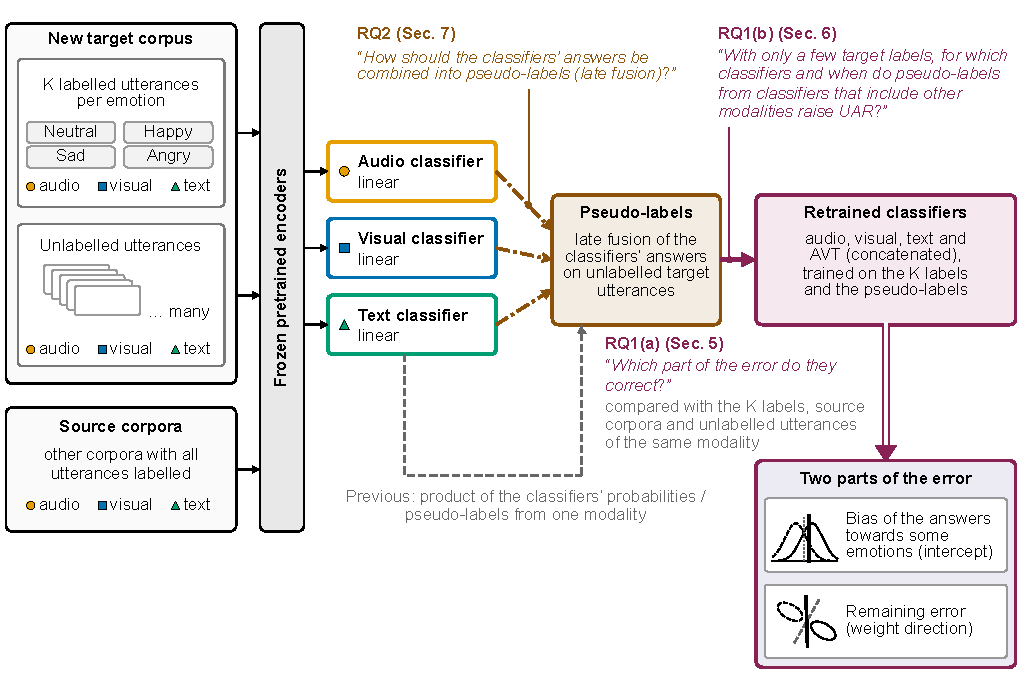
\includegraphics[width=0.74\linewidth]{fig1_questions.pdf}
\paperfig{1}{本研究の 3 つの問い（Q1〜Q3）と，それぞれに答える節．破線は従来の疑似ラベルの作り方を示す．}
\end{figure}
\vspace{-3pt}
\zumiru{左から右へ，データ → 凍結したエンコーダ → 声・顔・言葉の線形分類器 → 疑似ラベル → 学び直した分類器と流れ，問いの文は問う場所を指す細い線の先に書いてある．Q3 は疑似ラベルの作り方，Q1 は学び直した結果，Q2 は直した誤りの部分（右下の 2 つの箱）を問う．石井さんの論文（Ishii 2022 の Fig.~1）の「問いの概観」の図に倣った．図の語：Pseudo-labels ＝ 疑似ラベル，Retrained classifiers ＝ 学び直した分類器，Two parts of the error ＝ 誤りの 2 つの部分（Bias of the answers ＝ 答えの偏り，Remaining error ＝ 残りの誤り），Frozen pretrained encoders ＝ 凍結した事前学習エンコーダ，Previous ＝ 従来の方法．}

\noindent 論文 8 節の考察は，「8.1 Q1 への答え」「8.2 Q2 への答え」「8.3 Q3 への答え」と同じ番号に戻って答えをまとめる．

%======================================================================
\pagesection{道具：分類器の誤りを「答えの偏り」と「残りの誤り」に分ける}\label{sec:bunkai}
\koko[\ess{4}]{線形分類器の誤りを 2 つの部分に分けると，ある情報源が上げた UAR がどちらの部分を直した結果かを比べられる．}

\noindent 線形分類器は，感情 k ごとに点数 $s_k(x)=w_k^\top x+b_k$ を計算し，点数が最大の感情を答える（$x$ は特徴，$w_k$ は\textbf{重み}，$b_k$ は\textbf{切片}）．2 つの感情 k と l のどちらを答えるかは，点数の差 $z_{kl}=(w_k-w_l)^\top x+(b_k-b_l)$ が正か負かで決まる．この差を 1 本の数直線に並べると，誤りの 2 つの種類が見える（図 \ref{fig:toy}）．

\begin{figure}[H]
\centering
\begin{tikzpicture}[kd/.style={circle,fill=black,inner sep=1.7pt},ld/.style={circle,draw=black,fill=white,inner sep=1.7pt},er/.style={draw=cTest,thick,circle,minimum size=9pt,inner sep=0pt}]
  % (a)
  \begin{scope}
    \node[font=\small\bfseries,anchor=west] at (-3.2,1.55) {(a) 答えの偏り（切片のずれ）};
    \draw[->] (-3.1,0) -- (3.1,0) node[right,font=\scriptsize] {$z_{kl}$};
    \foreach \x in {0.4,0.9,1.4,1.9,2.4}{ \node[kd] at (\x,0.5) {}; }
    \foreach \x in {-2.4,-1.9,-1.4,-0.9,-0.4}{ \node[ld] at (\x,0.22) {}; }
    \foreach \x in {0.4,0.9}{ \node[er] at (\x,0.5) {}; }
    \draw[very thick] (1.15,-0.15) -- (1.15,1.05);
    \node[font=\scriptsize,anchor=west] at (1.2,1.0) {今の境目};
    \draw[dashed,black!60] (0,-0.15) -- (0,0.9);
    \node[font=\scriptsize,anchor=north] at (0,-0.12) {2 つの山の中点};
    \draw[-{Stealth},thick,cGood] (1.15,-0.62) -- (0.05,-0.62);
    \node[font=\scriptsize,cGood!70!black,anchor=west] at (1.25,-0.62) {切片を動かして境目を中点へ → 誤りは 0};
  \end{scope}
  % (b)
  \begin{scope}[xshift=9.0cm]
    \node[font=\small\bfseries,anchor=west] at (-3.2,1.55) {(b) 残りの誤り（重みの向きのずれ）};
    \draw[->] (-3.1,0) -- (3.1,0) node[right,font=\scriptsize] {$z_{kl}$};
    \foreach \x in {-0.6,0.2,0.9,1.5,2.2}{ \node[kd] at (\x,0.5) {}; }
    \foreach \x in {-2.2,-1.5,-0.9,-0.2,0.6}{ \node[ld] at (\x,0.22) {}; }
    \node[er] at (-0.6,0.5) {}; \node[er] at (0.6,0.22) {};
    \draw[very thick] (0,-0.15) -- (0,1.05);
    \node[font=\scriptsize,anchor=west] at (0.05,1.0) {境目（中点）};
    \node[font=\scriptsize,align=left,anchor=north] at (0,-0.2) {2 つの感情の発話が重なっているので，境目をどこに置いても\\誤りは 2 つより減らない．重みを変えないと直らない};
  \end{scope}
  \node[font=\scriptsize,anchor=west] at (-3.2,-1.25) {● 感情 k の発話　○ 感情 l の発話　{\color{cTest}赤い丸}：誤って答えた発話．境目より右なら k，左なら l と答える．値は説明用の例．};
\end{tikzpicture}
\caption{誤りの 2 つの種類（例）．}\label{fig:toy}
\end{figure}
\vspace{-4pt}
\begin{itemize}
  \item \textbf{答えの偏り（切片のずれ）}：境目が 2 つの山の中点からずれていて，答えが一方の感情に偏る誤りである．切片を動かせば直る．コーパスごとに特徴の平均がずれていること（すべての感情に共通のずれ）も，この部分だけを動かす．
  \item \textbf{残りの誤り（重みの向きのずれ）}：切片を一番よく選び直しても残る誤りである．2 つの感情の発話が点数の軸の上で重なっているために起こり，重み $w$ を変えないと直らない．
\end{itemize}

\begin{figure}[H]
\centering
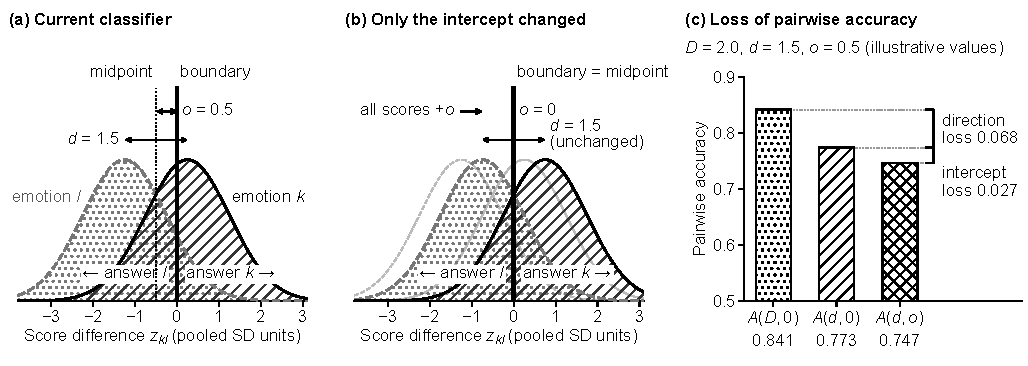
\includegraphics[width=0.9\linewidth]{fig2_decomposition.pdf}
\paperfig{2}{対の正解率の損は，切片を選び直しても残る向きの損と，切片で直せる切片の損に分かれる．(c) の値は説明のための例であり，結果ではない．}
\end{figure}
\vspace{-3pt}
\zumiru{(a) は今の分類器の $z_{kl}$ の上の 2 つの山で，$d$ は山の離れ方，$o$ は境目の中点からのずれである（どちらも山の標準偏差を 1 とした単位）．(b) は切片だけを変えた分類器で，$o$ は 0 になり $d$ は変わらない．(c) は 3 つの対の正解率で，$\Phi$ を標準正規分布の累積分布関数とすると $A(d,o)=\tfrac12[\Phi(d/2-o)+\Phi(d/2+o)]$ である．$D$ は最良の線形の向きでの山の離れ方．例の値（$D=2.0$，$d=1.5$，$o=0.5$）では，最良の向きと最良の切片の $A(D,0)=0.841$，今の向きと最良の切片の $A(d,0)=0.773$，今の分類器の $A(d,o)=0.747$ で，\textbf{向きの損}は 0.068，\textbf{切片の損}は 0.027 である（丸める前の値の差）．}

\noindent ターゲットのラベル，ほかのコーパス，ラベル無しの発話，ほかのモダリティの 4 つを同じ分け方で測ると，どの情報源がどちらの部分を直すかを比べられる（\ref{sec:q2all}〜\ref{sec:q2voice} 節）．評定を成分に分けてから「どの入力がどの成分を捉えたか」を測る Hayashi 2025（岡田先生・石井さんの共著）と同じ組み立てである．

%======================================================================
\pagesection{解析の設定，3 つの設定，数値の読み方}\label{sec:settei}
\koko{論文の分類器の作りと，結果を測った 3 つの設定を知ると，どの数値がどの設定のものかを読み違えない．}

\begin{waku}{解析のための設定（序論 5 段落目）}
\small
論文は，事前学習した\textbf{エンコーダ}（大量のデータで学習済みのネットワーク）を\textbf{凍結}して（中身を変えずに）使い，声・顔・言葉の発話を数の並び（\textbf{特徴}）に変える．その上に線形分類器を置く．この設定は新しい分類器の構造を提案するためではなく，情報源ごとに分類器の何が変わるかを測るための設定である．特徴の名前：A は声（WavLM-large．声だけ HuBERT-large でも計算），V は顔（ResNet-50 の表情モデル），T は言葉（RoBERTa-base），AV・VT・AT・AVT は特徴をつないだ融合の特徴．結果は凍結した特徴の上の線形分類器についてのもので，エンコーダを微調整する場合にまで広げては主張しない．
\end{waku}

\begin{figure}[H]
\centering
\begin{tikzpicture}[sb/.style={draw,rounded corners=2pt,align=center,font=\scriptsize,inner sep=3pt}]
  % 単一ソース
  \begin{scope}
    \node[font=\small\bfseries] at (2.6,2.55) {(a) 単一ソース設定};
    \node[sb,fill=cSrc!20,draw=cSrc!80!black,minimum width=2.2cm] (s) at (1.3,1.75) {ソース 1 群\\全発話のラベル};
    \node[sb,fill=cK!20,draw=cK!80!black,minimum width=2.2cm] (k) at (3.9,1.75) {ターゲット\\K 本};
    \node[sb,fill=black!5,minimum width=4.6cm] (m) at (2.6,0.5) {まとめて 1 つの分類器を学ぶ（\textbf{合併}）};
    \draw[arr] (s) -- (m); \draw[arr] (k) -- (m);
    \node[font=\scriptsize,align=center] at (2.6,-0.25) {比べる相手：K 本だけ，ソースだけ};
  \end{scope}
  % 全ソース
  \begin{scope}[xshift=5.9cm]
    \node[font=\small\bfseries] at (2.6,2.55) {(b) 全ソース設定};
    \node[sb,fill=cSrc!20,draw=cSrc!80!black,minimum width=2.2cm] (s) at (1.3,1.75) {ターゲット以外の\\全群};
    \node[sb,fill=black!5,minimum width=1.6cm] (an) at (1.3,0.5) {アンカー};
    \node[sb,fill=cK!20,draw=cK!80!black,minimum width=2.2cm] (k) at (3.9,1.75) {K 本と\\ラベル無し};
    \node[sb,fill=black!5,minimum width=2.0cm] (r) at (3.9,0.5) {学び直す};
    \draw[arr] (s) -- (an); \draw[arr] (an) -- (r); \draw[arr] (k) -- (r);
    \node[font=\scriptsize,align=center] at (2.6,-0.25) {疑似ラベルと同じモダリティの 8 手法を比べる};
  \end{scope}
  % LOCO
  \begin{scope}[xshift=11.8cm]
    \node[font=\small\bfseries] at (2.6,2.55) {(c) LOCO 設定};
    \foreach \nm/\x in {IEMOCAP/0.55,MOSEI/1.75,MELD/2.95}{ \node[sb,fill=cSrc!20,draw=cSrc!80!black,minimum width=1.1cm,font=\tiny] at (\x,1.8) {\nm}; }
    \node[sb,fill=cK!20,draw=cK!80!black,font=\tiny,minimum width=1.0cm] (t) at (4.4,1.8) {AFEW};
    \node[font=\tiny] at (1.75,2.18) {ソース 3 つ};
    \node[font=\tiny] at (4.4,2.18) {ターゲット};
    \node[sb,fill=black!5,minimum width=2.6cm] (an) at (1.75,0.6) {3 つのソースの分類器の\\平均 ＝ アンカー};
    \node[sb,fill=black!5,minimum width=1.5cm] (r) at (4.4,0.6) {K 本と疑似\\ラベルで\\学び直す};
    \draw[arr] (1.75,1.55) -- (an); \draw[arr] (an) -- (r); \draw[arr] (t) -- (r);
    \node[font=\scriptsize,align=center] at (2.6,-0.25) {4 コーパスを 1 つずつターゲットにする};
  \end{scope}
\end{tikzpicture}
\caption{3 つの設定．LOCO は leave-one-corpus-out（1 つのコーパスを抜いてターゲットにする）の略．(c) は AFEW がターゲットの場合．}
\end{figure}
\vspace{-4pt}
\begin{center}
\small
\begin{tabular}{>{\raggedright}p{2.3cm}>{\raggedright}p{7.0cm}p{2.4cm}p{1.8cm}p{1.8cm}}
\toprule
設定 & ソースの使い方 & K & 論文の節 & この資料 \\
\midrule
単一ソース設定 & 1 つのソースの群の全発話とターゲットの K 本をまとめて学ぶ（7 群．IEMOCAP の即興と台本は別の群） & 1，5，10，25，50，全件 & 6.1〜6.3 & \ref{sec:q2mix}・\ref{sec:q2bias} 節 \\
全ソース設定 & ターゲット以外の全群で学んだ分類器をアンカーにし，K 本で学び直す & 0，5，25 & 6.4 & \ref{sec:q2pl} 節 \\
LOCO 設定 & 4 コーパスの 1 つをターゲット，残る 3 つをソースにし，3 つのソースの分類器の平均をアンカーにする（論文 7 節は CREMA-D も評価） & 0，5，10，25 & 5，6.5，6.6，7 & \ref{sec:q1how}〜\ref{sec:q1cont}，\ref{sec:q2cond}〜\ref{sec:q3cont} 節 \\
\bottomrule
\end{tabular}
\end{center}
\noindent\textbf{アンカー}は，学び直すときに重みと切片を引き戻す先の分類器である．重みと切片がアンカーから離れるほど損失に罰を足す（\textbf{L2 正則化}）．

\begin{waku}{テストのラベルでハイパーパラメータを選ばない}
\small LOCO 設定では，評価のターゲット以外の 3 コーパスを 1 つずつ\textbf{仮のターゲット}にして（ソースは残る 2 つ）ハイパーパラメータ（学習の前に決めておく数）を選んで固定し（\textbf{仮のターゲットの回}．30 反復），その後，評価のターゲットで 1 回だけ計算した（\textbf{評価の回}．50 反復）．テストの発話の正解は，成績を測るときにだけ使う．
\end{waku}

\noindent\textbf{数値の読み方}
\begin{itemize}
  \item \textbf{gain}：2 つの方法の UAR の差（点）．何との差かを括弧に書く．例：gain（合併 − K 本だけ）．
  \item \textbf{95\% 区間}：テストに入る話者（MOSEI と LOCO 設定では話者の代わりのまとまりである\textbf{クラスタ}）の取り方と，K 本の抜き方による揺れを表す．区間が 0 をまたがなければ，この揺れを考えても差の符号は変わらないと読む．ソースのコーパスの選び方，学習に使う発話，手法の選び方による揺れは含まない．
  \item \textbf{条件}はコーパス × 分類器 × K のような 1 つの組み合わせ，\textbf{反復}は分割 × K 本の引き方の 1 回である（評価の回は 5 分割 × 10 種 = 50 反復）．
  \item \textbf{話者を分ける}：同じ話者の発話が，学習に使う発話と評価に使う発話の両方に入らないように分けた．MOSEI には話者の注釈が無いので，チャンネルか動画で分けた（同じ人物の別の動画が両方に入りうる）．
\end{itemize}

%======================================================================
\pagesection{Q1：どう測ったか（融合の疑似ラベルによる学び直し）}\label{sec:q1how}
\toihead[\ess{3}]{cQ1}{Q1}{新しいコーパスに感情ごとに数本のラベルしか無いとき，ほかのモダリティの疑似ラベルで学び直すと，声・顔・言葉の分類器の UAR は上がるか．}

\noindent LOCO 設定で，ターゲットの発話のうちテストに入らないものを\textbf{候補}と呼ぶ．候補から感情ごとに K 本を抜いてラベルを使い，ほかの候補のラベルは使わない．疑似ラベル q は次の手順で作り，それを使って各分類器を学び直す（図 \ref{fig:pipeline}）．

\begin{figure}[H]
\centering
\begin{tikzpicture}[pb/.style={draw,rounded corners=2pt,align=center,font=\scriptsize,inner sep=4pt,text width=3.3cm,minimum height=1.55cm}]
  \node[pb,fill=black!5] (a) at (0,0) {\textbf{(1) アンカー}\\3 つのソースのコーパスで学んだ分類器の重みと切片の平均};
  \node[pb,fill=cF!8] (b) at (4.25,0) {\textbf{(2) K 本だけの融合の分類器}\\声・顔・言葉をつないだ特徴（AVT）．候補に確率を付ける};
  \node[pb,fill=cA!12] (c) at (8.5,0) {\textbf{(3) 声・顔・言葉の分類器}\\アンカーから，K 本と (2) の確率で学び直す};
  \node[pb,fill=cQ3!10,draw=cQ3!80!black] (d) at (12.75,0) {\textbf{(4) 疑似ラベル q}\\(3) の 3 つの確率を発話ごとに掛け，足して 1 になるように直す（\textbf{積}）};
  \node[pb,fill=cQ1!8,draw=cQ1!80!black,text width=10.5cm,minimum height=1.25cm] (e) at (7.75,-2.3) {\textbf{(5) 学び直し}：声・顔・言葉・融合の各分類器を，アンカーから K 本と q で学び直す\\損失 ＝（K 本の交差エントロピー）＋（候補の q との交差エントロピー）＋（アンカーへの L2 正則化）};
  \draw[arr] (a) -- (b); \draw[arr] (b) -- (c); \draw[arr] (c) -- (d);
  \draw[arr] (d.south) -- (d.south |- e.north);
  \node[pb,fill=white,draw=black!50,text width=3.4cm,minimum height=1.25cm] (f) at (0,-2.3) {\textbf{比べる基準}\\K 本だけの分類器（アンカーから K 本だけで学び直す）};
\end{tikzpicture}
\caption{融合の疑似ラベルによる学び直し（論文 5.1 節）．K = 0 では，K 本だけの分類器はアンカーそのものである．}\label{fig:pipeline}
\end{figure}

\begin{itemize}
  \item \textbf{交差エントロピー}は，分類器の確率が目標（正解か q）から離れるほど大きくなる量で，学習はこれを小さくする．
  \item 損失は 2 つの形で解いた．\textbf{形 (a)} は疑似ラベルの重みの合計を感情ごとにそろえる．\textbf{形 (b)} は温度つきの交差エントロピー（Hinton ほか 2015 の蒸留の損失．温度 τ = 2 は Albanie ほか 2018 の値）である．この資料で「学び直し」と書くときは形 (a) を指す．
  \item q は，学び直す分類器自身のモダリティの予測も含む．
  \item ハイパーパラメータ（疑似ラベルの重み ρ，K 本の倍率 a，積の指数）は仮のターゲットの 30 反復で選んで固定した．調整しないときの値は ρ = 1，a = 1，指数 (1, 1, 1) である．
\end{itemize}

\noindent\textbf{比べる手法は 2 組ある}（論文 5.2 節）．
\begin{enumerate}
  \item q を受け取るほかの損失の形 5 つ：形 (b)，一致した発話だけの疑似ラベル，自分の予測と混ぜる方法（Zhang ほか 2021），柔らかい共訓練，共正則化．どれも原論文の損失を q を受け取るように移した版である．80 条件のうち 75 で形 (b) が仮のターゲットで選ばれた．
  \item q を使わない 11 手法：同じモダリティのラベル無しの発話か，ソースのラベル付きの発話を使う（自己学習，エントロピー最小化，IM，T3A，ラベル伝播，自分の予測を形 (a) で使う版，S+T，CORAL，DANN，MME，xMUDA 型）．
\end{enumerate}
\noindent どの手法も同じアンカーと K 本から学び，ハイパーパラメータを同じ手順で選んだ．値は 5 分割 × K 本の抜き方 10 種の 50 反復の平均である（K = 0 は 5 反復）．

%======================================================================
\pagesection{Q1 の答え：声の分類器の UAR は 12 条件すべてで上がった}\label{sec:q1ans}
\toihead{cQ1}{Q1}{ほかのモダリティの疑似ラベルで学び直すと，分類器の UAR は上がるか．}
\begin{kotae}{cQ1}{Q1 の答え（論文 5 節の冒頭）}
LOCO 設定でほかのモダリティを含む疑似ラベルにより学び直すと，声の分類器の UAR は，4 コーパス × 3 つの K（0，5，25）の 12 条件すべてで点推定が K 本だけの分類器を上回り，K = 5 では 2.4〜4.1 点上がった．12 条件のうち 10 では 95\% 区間の下端が 0 を超えた．\par
{\small（K = 5 は，感情ごとに 5 本，計 20 本のラベルがある条件である．）}
\end{kotae}

\begin{figure}[H]
\centering
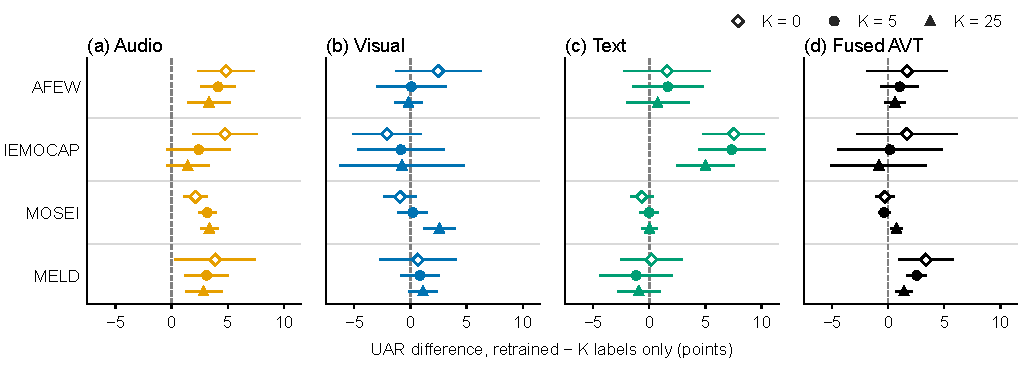
\includegraphics[width=\linewidth]{fig3_q1_retraining.pdf}
\paperfig{3}{融合の疑似ラベルで学び直すと，声の分類器の UAR は 4 コーパスと 3 つの K のすべてで上がり，顔・言葉・融合の分類器では上がったコーパスが限られた．}
\end{figure}
\vspace{-3pt}
\zumiru{各点は gain（学び直した分類器 − K 本だけの分類器）で，破線の 0 より右なら学び直しで上がった．横の棒は 95\% 区間である．印はひし形が K = 0，丸が K = 5，三角が K = 25．パネルは (a) 声，(b) 顔，(c) 言葉，(d) 融合（AVT）．(a) の声では 12 個の点がすべて 0 より右にある．}

\begin{center}
\small
\begin{tabular}{lcccc}
\toprule
声の分類器，K = 5 & K 本だけ & 学び直し & gain（学び直し − K 本だけ）[95\% 区間] & K = 0，5，25 の gain の範囲 \\
\midrule
AFEW & 50.1 & 54.2 & +4.15 [+2.56, +5.74] & +3.3〜+4.9 \\
IEMOCAP & 67.1 & 69.5 & +2.41 [−0.45, +5.27] & +1.4〜+4.8 \\
MOSEI & 34.9 & 38.1 & +3.19 [+2.38, +3.99] & +2.1〜+3.4 \\
MELD & 41.5 & 44.6 & +3.12 [+1.18, +5.06] & +2.9〜+3.9 \\
\bottomrule
\end{tabular}
\end{center}
\noindent 声の gain は，候補の全ラベルで学べば得られる上がり幅（余地．\shiryo{sec:q2cond}）の 24\%（IEMOCAP）〜67\%（AFEW）だった．

\begin{yowai}
\begin{itemize}
  \item 声でも，IEMOCAP の K = 5 と K = 25 は区間が 0 を含んだ（K = 5 は +2.41 [−0.45, +5.27]）．
  \item 検定は，計算の前に差を検出できる見込みがあると判定した 15 条件に限った．MOSEI の 3 条件は Holm の補正（たくさん検定したぶんだけ基準を厳しくする手続き）の後も有意で（p < 0.001），MELD の K = 0，5 は有意ではなかった（p = 0.27，0.06）．
  \item 顔・言葉・融合の分類器で区間の下端が 0 を超えた条件は，12 条件のうちそれぞれ 1，3，4 だった．言葉は IEMOCAP で +5.0〜+7.5 点，融合は MELD で +1.4〜+3.4 点上がったが，顔は IEMOCAP の 3 つの K で差が負だった（−2.1〜−0.7．区間は 0 を含む）．分類器で違った理由は \shiryo{sec:q2cond}で調べる．
  \item q は学び直す分類器自身のモダリティの予測も含むので，gain をほかのモダリティの情報だけに帰すことはできない（論文 9 節）．
\end{itemize}
\end{yowai}

%======================================================================
\pagesection{Q1 の答え（続き）：上がり幅は損失の形によらず，疑似ラベルを使わない手法は低かった}\label{sec:q1cont}
\koko{声の gain が損失の細かい形やハイパーパラメータの選び方から生じたのではないことと，疑似ラベルを使わない手法では同じだけ上がらなかったことを示す．}

\noindent\textbf{損失の形とハイパーパラメータの選択によらなかった}（論文 5.5 節）．
\begin{itemize}
  \item 形 (a) − 1 組目で選ばれた形（48 条件のうち 45 で形 (b)）の区間は，K = 0，5，25 の 48 条件のうち 40 で 0 を含んだ．声の 12 条件の差は −0.79〜+0.88 点だった．0 を含まなかった 8 条件のうち 7 は言葉の分類器（5 条件）か MOSEI の声（2 条件）で，差は −1.24〜−0.16 点だった．
  \item 仮のターゲットで選んだ形 (a) のハイパーパラメータは，48 条件のうち 44（声は 12 条件すべて）で調整しないときの値と同じ分類器になった．
\end{itemize}
論文はここで「示す」ではなく「示唆する」を使う：「これらの結果は，表 4 の声の gain が，損失の形にも仮のターゲットでのハイパーパラメータの選択にもよらず，学び直す分類器の損失に q を加えることから生じたことを示唆する．」（測った結果からの解釈なので「示唆する」．\shiryo{sec:doushi}）

\medskip
\noindent\textbf{q を使わない手法は，声の分類器で学び直しより低い UAR だった}（論文の表 5 の声の列）．
\begin{center}
\small
\begin{tabular}{lcccc}
\toprule
声の分類器，K = 5 の UAR & AFEW & IEMOCAP & MOSEI & MELD \\
\midrule
\rowcolor{cQ1!8} 学び直し（形 (a)．参考） & 54.2 & 69.5 & 38.1 & 44.6 \\
K 本だけ（参考） & 50.1 & 67.1 & 34.9 & 41.5 \\
\midrule
自己学習 & 50.1* & 67.1 & 32.0* & 40.7* \\
エントロピー最小化 & 31.8* & 38.4* & 25.0* & 26.9* \\
IM & 50.6* & 66.8* & 34.6* & 40.5* \\
T3A & 44.3* & 57.1* & 30.7* & 34.0* \\
ラベル伝播 & 45.3* & 58.6* & 32.3* & 31.0* \\
自分の予測を形 (a) で使う版 & 50.6* & 66.8 & 35.0* & 41.9* \\
S+T（ソースのラベル付きの発話と K 本を合わせて学ぶ） & 50.2* & 62.1* & 35.5* & 41.1* \\
CORAL & 49.3* & 64.4* & 35.2* & 41.0* \\
DANN & 46.5* & 64.6* & 34.5* & 39.3* \\
MME & 46.5* & 63.4* & 30.8* & 33.3* \\
xMUDA 型（相互の模倣） & 48.8* & 68.9 & 35.7* & 37.5* \\
\bottomrule
\end{tabular}

\smallskip
{\footnotesize * は「学び直し − その手法」の 95\% 区間の下端が 0 を超えたことを示す．値は 50 反復の平均（DANN，MME，xMUDA 型は 15 反復）．}
\end{center}
\begin{itemize}
  \item 11 手法 × 4 コーパスの 44 の比べで，学び直し − 手法は +0.7〜+31.0 点だった．区間の下端が 0 を超えなかったのは IEMOCAP の 3 つ（自己学習，自分の予測を形 (a) で使う版，xMUDA 型）だけである．K = 0，5，25 の 128 の比べでも差はすべて正だった．
  \item 論文の読み方：これらの手法は q と違う情報（同じモダリティのラベル無しの発話，ソースのラベル付きの発話）を使うので，差は手法の優劣ではなく使う情報の違いとして読む．
  \item 融合の分類器では，区間の下端が 0 を超えた条件は手法ごとに 12 条件のうち 3〜9 で，上端が 0 を下回った条件も 4 つあった．
\end{itemize}
\noindent 次の Q2 では，q による学び直しで分類器の誤りのどの部分が減ったのかを調べる．

%======================================================================
\pagesection{Q2 の答え（全体）：疑似ラベルが直したのは，答えの偏りを除いても残る誤りだった}\label{sec:q2all}
\toihead[\ess{4}]{cQ2}{Q2}{上がるなら，分類器の誤りのどの部分が直るのか．ターゲットのラベル，ほかのコーパス，同じモダリティのラベル無しの発話とは，直す部分がどう違うのか．そして，どの分類器で上がるのか．}

\begin{kotae}{cQ2}{Q2 の答え（論文 6 節の冒頭）}
ほかのモダリティを含む疑似ラベルが減らしたのは，答えが一部の感情に偏る誤り（切片のずれ）ではなく，偏りを除いても残る誤り（重みの向きのずれ．以下，残りの誤り）だった．偏りは K 本でもラベル無しで特徴の平均を引いても直ったが，残りの誤りは K 本では遅くしか直らず，同じモダリティのラベル無しの発話ではほとんど減らなかった．UAR が上がったのは，余地があり，疑似ラベルが当たり，その判断を自分の特徴で再現できる分類器で，評価で 3 つの量を測った声・顔・言葉の分類器のうち，4 コーパスで 3 つの点推定がすべて正だったのは声の分類器だった．
\end{kotae}

\noindent Q1 で「上がった」を示した後に，Q2 で「なぜ上がったか」を誤りの 2 つの部分に分けて答える．下の表は，4 つの情報源が 2 つの部分のどちらを直したかを 1 枚にまとめたものである．

\begin{center}
\small
\begin{tabular}{>{\raggedright}p{4.1cm}>{\raggedright}p{3.6cm}>{\raggedright}p{6.1cm}p{1.3cm}}
\toprule
情報源 & 分かったこと & 数値（論文の値） & 資料 \\
\midrule
\chip{cSrc}{ソース}\ ほかのコーパスを 1 つ混ぜる（単一ソース設定） & K が小さいときだけ gain が正 & gain（合併 − K 本だけ）は K = 1 で 8 種類の特徴すべてで正（6.9〜13.4 点），全件で 8 種類すべてで負（−2.1〜−4.8 点） & \ref{sec:q2mix} 節 \\
\chip{cK}{K 本}\ 合併の中のターゲットの K 本 & 主に\textbf{答えの偏り}を直した & 切片だけの直しで合併の gain の 0.91 倍（声，WavLM，K = 5） & \ref{sec:q2bias} 節 \\
\chipk{cU}{ラベル無し}\ 特徴の平均を引く & \textbf{答えの偏り}を直した & +4.69 点（合併は +5.26 点．声，WavLM，K = 5） & \ref{sec:q2bias} 節 \\
\chip{cK}{K 本}\ K 本だけで学ぶ & \textbf{残りの誤り}は遅くしか直らない & 重みの向きの良さ（最良の向きを 1 とした比）は声で K = 5 で 0.47，K = 10 で 0.62 & \ref{sec:q2bias} 節 \\
\chipk{cU}{ラベル無し}\ 同じモダリティのラベル無しの発話を使う 8 手法 & \textbf{残りの誤り}をほとんど減らさない & 210 条件のうち 7 で減らし，79 で増やした & \ref{sec:q2pl} 節 \\
\chip{cQ1}{ほかのモダリティ}\ ほかのモダリティを含む疑似ラベル & \textbf{残りの誤り}を減らした & 81 条件のうち 38 で減らし，1 で増やした & \ref{sec:q2pl} 節 \\
\bottomrule
\end{tabular}
\end{center}

\noindent\textbf{どの分類器で上がるか}：学び直しで UAR が上がったのは，次の 3 つの条件がそろう分類器だった（\shiryo{sec:q2cond}）．
\begin{center}
\begin{tikzpicture}[cb/.style={draw,rounded corners=3pt,align=center,font=\small,inner sep=5pt,minimum height=1.3cm,text width=3.6cm}]
  \node[cb,fill=cQ2!6] (a) at (0,0) {\textbf{① 余地がある}\\伸びしろがある};
  \node[cb,fill=cQ2!6] (b) at (4.6,0) {\textbf{② 疑似ラベルが当たる}\\今の分類器より当たる};
  \node[cb,fill=cQ2!6] (c) at (9.2,0) {\textbf{③ 自分の特徴で再現できる}\\q の判断を自分の特徴で学べる};
  \node[cb,fill=cGood!12,draw=cGood!70!black,text width=2.6cm] (d) at (13.5,0) {学び直しで\\UAR が上がる};
  \node[font=\Large] at (2.3,0) {＋}; \node[font=\Large] at (6.9,0) {＋};
  \draw[arr] (c) -- (d);
\end{tikzpicture}
\end{center}
\noindent 声の分類器で ③ が満たされた理由の候補として，声の特徴は言葉の分類器の判断を顔の特徴より 14.9〜16.7 点よく再現した（\shiryo{sec:q2voice}）．

%======================================================================
\pagesection{Q2 の答え (1)：ほかのコーパスを混ぜる gain は，K が小さいときだけ正だった}\label{sec:q2mix}
\toihead{cQ2}{Q2}{ターゲットのラベルの本数 K によって，ほかのコーパスのラベル付きの発話を混ぜたときの UAR の上がり方はどう変わるか．}

\noindent 単一ソース設定で，ソースのコーパス 1 つのラベル付きの全発話とターゲットの K 本をまとめて 1 つの分類器（合併）を学び，テストの UAR の差を gain（合併 − K 本だけ）とした．gain は特徴ごとに，群のすべての順序つきの組（IEMOCAP の即興と台本の組を除く 10〜40 組）で平均した．

\begin{figure}[H]
\centering
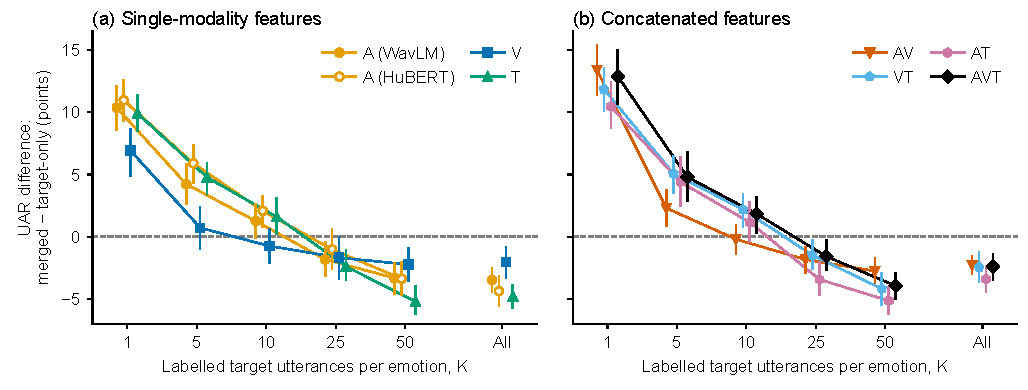
\includegraphics[width=\linewidth]{fig4_mixing_gain.pdf}
\paperfig{4}{ソースのコーパスを 1 つ混ぜる gain は，K = 1 で 8 種類の特徴すべてで正で，K が増えると小さくなり，ターゲットの全ラベルを使うと 8 種類すべてで負だった．}
\end{figure}
\vspace{-3pt}
\zumiru{横軸はターゲットの感情ごとのラベルの本数 K，縦軸は gain（合併 − K 本だけ）である．点が破線の 0 より上ならソースを混ぜると上がり，下なら下がる．右端の All はターゲットの学習用のラベルを全部使った場合である．図の語：(a) Single-modality features ＝ 1 つのモダリティの特徴，(b) Fused features ＝ 融合の特徴．}

\begin{center}
\small
\begin{tabular}{lll}
\toprule
K & 平均の gain の範囲（8 種類の特徴） & 95\% 区間の例 \\
\midrule
1 & V の 6.9 点 〜 AV の 13.4 点 & V 4.8〜8.7，AV 11.4〜15.4 \\
5 & V の 0.7 点 〜 A（HuBERT）の 5.9 点 & V −1.0〜2.4，A（HuBERT）4.3〜7.4 \\
全件 & V の −2.1 点 〜 T の −4.8 点 & 8 種類すべてで区間が 0 より下 \\
\bottomrule
\end{tabular}
\end{center}

\begin{yowai}
全件での損は，多くの組に共通してはいなかった．組ごとの判定で，Holm の補正の後に負だった組は A（WavLM）で 40 組のうち 5 だった．図の点は組の平均である．
\end{yowai}

\noindent\textbf{論文の解釈}（8.2 節）：合わせて学ぶ中で数本のラベルがしていた仕事が主に答えの偏りの直しなら，ターゲットのラベルが増えれば偏りはターゲットだけでも直り，ソースの発話が足すものは少なくなる．この「数本のラベルがしていた仕事」を次の頁で測る．

%======================================================================
\pagesection{Q2 の答え (2)：K 本の仕事は主に答えの偏りの直しで，残りの誤りは K 本では遅くしか直らなかった}\label{sec:q2bias}
\toihead{cQ2}{Q2}{合併の中でターゲットの K 本は何を直していたのか．残りの誤りは K 本でどれだけ直るのか．}

\noindent 単一ソース設定の K = 5 で，ソースの全発話だけで学んだ分類器（\textbf{ソースだけ}）に対する gain を比べた．\textbf{切片だけの直し}は，ソースだけの分類器の重みを固定し，4 つの切片に足すずらしだけを K 本で学ぶ．\textbf{平均を引く方法}は，ソースとターゲットの特徴からそれぞれの全発話の平均を引いてソースだけの分類器を学び直し，ターゲットのラベルを使わない．どちらの操作も残りの誤り（向きの損）を変えない（\shiryo{sec:bunkai}）．

\begin{figure}[H]
\centering
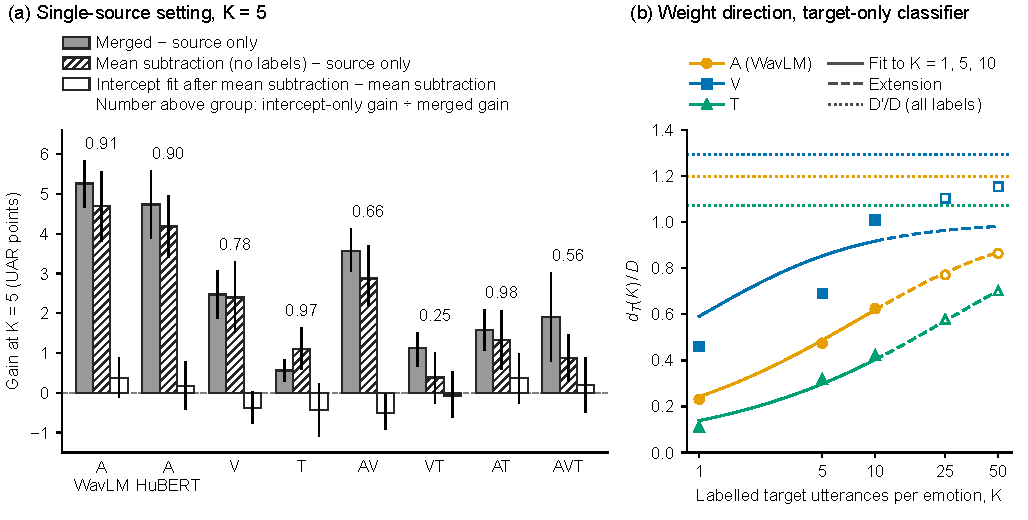
\includegraphics[width=0.8\linewidth]{fig5_bias_and_direction.pdf}
\paperfig{5}{合併の中で K 本がしていた仕事は主に偏りの直しで，残りの誤りは K を増やしても遅くしか直らなかった．}
\end{figure}
\vspace{-3pt}
\zumiru{(a) 灰色の棒は合併の gain，斜線の棒はラベルを使わずに特徴の平均を引いた方法の gain（どちらもソースだけとの差）で，2 本がほぼ同じ高さなら，ラベル無しで合併とほぼ同じだけ上がったと読む．白い棒は，平均を引いた後に K 本で切片を直した上乗せ．棒の上の数は「切片だけの直しの gain ÷ 合併の gain」．(b) 縦軸 $d_T(K)/D$ は K 本だけで学んだ分類器の重みの向きの良さ（最良の線形の向きを 1 とした比）で，点線は全ラベルで学んだ同じ分類器の値．}

\begin{itemize}
  \item 切片だけの直しの gain ÷ 合併の gain は，A（WavLM）で 0.91，A（HuBERT）で 0.90，V で 0.78 だった．
  \item 平均を引く方法は，ターゲットのラベルを使わずに合併に近い gain を得た．A（WavLM）では +4.69（+3.81〜+5.57）で合併の +5.26 との差は 0.57，V では +2.40 で合併の +2.47 との差は 0.07 だった．平均を引いた後に K 本で切片を直した上乗せは A（WavLM）で +0.38（−0.12〜+0.88）で，8 種類のどれでも区間が 0 より上にならなかった．
  \item K 本だけの分類器の向きの良さ $d_T/D$ は，A（WavLM）で K = 1，5，10 のとき 0.23，0.47，0.62，T で 0.11，0.32，0.42 だった．全ラベルで学んだ同じ分類器を基準にしても，K = 10 の離れ方は A（WavLM）で 0.53 倍，T で 0.40 倍だった．顔は速く，V は K = 10 で 1.01 に達した．
\end{itemize}

\begin{yowai}
0.91 などの比は 2 つの学習器の gain の比であり，合併の gain を偏りの分と残りの分に分けた割合ではない．切片のずらしの正則化の係数を 0.1 にするか，テストを除いた平均を使うと，A（WavLM）の上乗せの区間は 0 より上になった．(b) の曲線は K $\le$ 10 の範囲の要約で，計算の前に決めた仮定のうち 2 つは満たされなかった（論文 9 節）．
\end{yowai}

\begin{setsu}{この結果が Q3 の手法の形を決めた（論文 6.3 節の最後）}
K 本が直すのは主に答えの偏りで，重みの向きは K 本では遅くしか良くならない．そこで論文 7 節の手法では，分類器の信頼度を切片に依らない量で定義し，K 本からは分類器ごとに 1 つの数（水準）だけを測る（\shiryo{sec:q3mot}）．
\end{setsu}

%======================================================================
\pagesection{Q2 の答え (3)：ほかのモダリティの疑似ラベルは残りの誤りを減らした}\label{sec:q2pl}
\toihead{cQ2}{Q2}{ほかのモダリティの疑似ラベルと，同じモダリティのラベル無しの発話を使う方法は，残りの誤りをどれだけ減らすか．}

\noindent 全ソース設定で，ターゲット以外の全群で学んだ分類器をアンカーにし，K 本で学び直した分類器（全ソース設定の K 本だけ）を基準にした．疑似ラベルによる学び直しは，この損失に疑似ラベルとの交差エントロピーを足す．疑似ラベルは条件ごとに仮のターゲットで選び，102 の選択のうち 95 が各モダリティの分類器の確率の積だった．声・顔・言葉の組（AVT．3 コーパス）と声・顔の組（AV．5 コーパス）で，K = 0，5，25 の 81 条件になる．比べる相手は同じモダリティのラベル無しの発話を使う 8 手法（エントロピー最小化，自己学習，IM，T3A，ラベル伝播，CORAL，DANN，MME）の 210 条件である．

\noindent\textbf{判定の規則（計算の前に決めた）}：「K 本だけの向きの損 − 手法の向きの損」の 95\% 区間が 0 より上で，点の値が δ 以上なら「減らした」，0 より下で −δ 以下なら「増やした」．δ（0.82〜1.11 点）は仮のターゲットの出力だけから決めた．

\begin{figure}[H]
\centering
\begin{tikzpicture}
  \def\WW{11.0}
  % 疑似ラベル 81
  \node[font=\small,anchor=east,align=right] at (-0.15,1.2) {ほかのモダリティを含む\\疑似ラベル（81 条件）};
  \pgfmathsetmacro{\uu}{\WW/81}
  \fill[cGood] (0,0.95) rectangle ++(38*\uu,0.5); \node[font=\scriptsize\bfseries,white] at (19*\uu,1.2) {減らした 38};
  \fill[black!25] (38*\uu,0.95) rectangle ++(7*\uu,0.5); \node[font=\scriptsize] at (41.5*\uu,1.2) {7};
  \fill[cTest] (45*\uu,0.95) rectangle ++(1*\uu,0.5);
  \draw[pattern=north east lines,pattern color=black!35] (46*\uu,0.95) rectangle ++(35*\uu,0.5); \node[font=\scriptsize,fill=white,inner sep=1pt] at (63.5*\uu,1.2) {判定できない 35};
  \node[font=\scriptsize,cTest,anchor=south] at (45.5*\uu,1.45) {増やした 1};
  % 8 手法 210
  \node[font=\small,anchor=east,align=right] at (-0.15,0.0) {同じモダリティの\\8 手法（210 条件）};
  \pgfmathsetmacro{\vv}{\WW/210}
  \fill[cGood] (0,-0.25) rectangle ++(7*\vv,0.5);
  \node[font=\scriptsize,cGood!70!black,anchor=north west] at (0.02,-0.27) {減らした 7};
  \fill[black!25] (7*\vv,-0.25) rectangle ++(60*\vv,0.5); \node[font=\scriptsize] at (37*\vv,0) {同じ水準 60};
  \fill[cTest] (67*\vv,-0.25) rectangle ++(79*\vv,0.5); \node[font=\scriptsize\bfseries,white] at (106.5*\vv,0) {増やした 79};
  \draw[pattern=north east lines,pattern color=black!35] (146*\vv,-0.25) rectangle ++(48*\vv,0.5); \node[font=\scriptsize,fill=white,inner sep=1pt] at (170*\vv,0) {判定できない 48};
  \fill[black!55] (194*\vv,-0.25) rectangle ++(16*\vv,0.5); \node[font=\scriptsize,white] at (202*\vv,0) {16};
  \node[font=\scriptsize,anchor=north,align=center] at (202*\vv,-0.27) {働かな\\かった};
  \draw[black!40] (0,-0.5) -- (0,1.6); \draw[black!40] (\WW,-0.5) -- (\WW,1.6);
\end{tikzpicture}
\caption{向きの損（残りの誤り）の判定の数（論文の表 6）．帯の長さは各行の条件の数の割合で，中の数は条件の数．灰色は「同じ水準」，斜線は「判定できない」．「働かなかった」は，DANN と MME の適応の項が予測を変えた量が種の違いによる揺れと見分けられなかった条件である．}
\end{figure}

\begin{center}
\small
\begin{tabular}{llcl}
\toprule
組 & 学び直した分類器 & 条件 & 向きの損：減らした／同じ水準／増やした／判定できない \\
\midrule
AVT & \textcolor{cA}{\textbf{声}} & 9 & \textbf{9}／0／0／0 \\
AVT & \textcolor{cV}{\textbf{顔}} & 9 & 1／1／0／7 \\
AVT & \textcolor{cT}{\textbf{言葉}} & 9 & 5／0／1／3 \\
AVT & 融合 & 9 & 6／1／0／2 \\
AV & \textcolor{cA}{\textbf{声}} & 15 & 7／0／0／8 \\
AV & \textcolor{cV}{\textbf{顔}} & 15 & 5／0／0／10 \\
AV & 融合 & 15 & 5／5／0／5 \\
\bottomrule
\end{tabular}
\end{center}
\begin{itemize}
  \item 差が 0 のときに偶然に「減らした」となる条件の数の見込みは，81 条件で 2.02，210 条件で 5.25 である．
  \item UAR は 81 条件のうち 32 で K 本だけの分類器を上回り，下回った条件は無かった．
  \item 同じアンカー・同じ条件（AVT と AV の組，K = 0 と 5）で測った点の値では，373 対のうち 341 対で疑似ラベルによる学び直しのほうが向きの損を多く減らした．δ を半分にすると減らした条件は 81 のうち 49，2 倍にすると 20 だった．
\end{itemize}
\begin{yowai}
81 条件と 210 条件は同じ条件の上の比べではない．210 条件には融合の分類器と K = 25 が入らず，アンカーも違う．81 条件のうち 35 は「判定できない」だった．疑似ラベルはどれも学び直す分類器自身のモダリティの予測を含む．
\end{yowai}

%======================================================================
\pagesection{Q2 の答え (4)：UAR が上がったのは，3 つの条件がそろう分類器だった}\label{sec:q2cond}
\toihead{cQ2}{Q2}{同じ疑似ラベルで学び直しても，上がる分類器と上がらない分類器があったのはなぜか．}

\noindent LOCO 設定（Q1 と同じ計算）で，上がる条件として 3 つの量を置き，どれも UAR の差（点）で測った．

\noindent
\begin{minipage}[t]{0.44\linewidth}
\vspace{0pt}
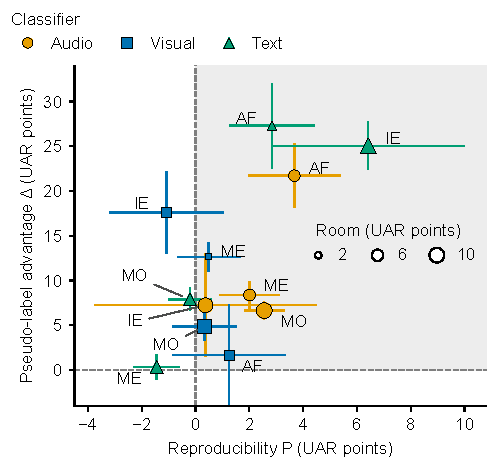
\includegraphics[width=\linewidth]{fig6_conditions.pdf}
\end{minipage}\hfill
\begin{minipage}[t]{0.535\linewidth}
\vspace{0pt}
\small
\textbf{① 余地}：候補の全ラベルで学べばどこまで上がるか．候補の全ラベルで学んだ重みに，テストの感情の割合で切片を当て直した分類器 − K 本だけの分類器（テストの上）．

\smallskip
\textbf{② 当たる幅 Δ}：疑似ラベル q がどれだけ当たるか．K 本を除いた候補の上で，q の答えの UAR − K 本だけの分類器の UAR．

\smallskip
\textbf{③ 再現できる分 P}：q の判断を，学び直す分類器と同じ特徴（たとえば声の特徴）だけでどれだけ学べるか．その特徴で q の答えを目標に学んだ線形分類器の UAR（候補を 2 組に分けた交差の予測）− 同じ発話の上の K 本だけの分類器．

\smallskip
{\textbf{論文の図 6（左）．}評価で 3 つの量を測った声・顔・言葉の分類器のうち，3 つの量の点推定が 4 コーパスすべてで正だったのは声の分類器だった．}
\end{minipage}

\zumiru{横軸は P，縦軸は Δ，印の大きさは余地（K = 5）．灰色の領域（P と Δ がともに正）に入るほど 3 つの条件がそろう．丸（Audio）が声，四角（Visual）が顔，三角（Text）が言葉，AF・IE・MO・ME はコーパスの頭文字．声の丸は 4 つとも P と Δ が正の位置にあり，顔の四角は P が 0 に近い．融合の分類器は載せていない．}

\begin{center}
\footnotesize
\begin{tabular}{llrrrllr}
\toprule
分類器 & コーパス & 余地 & K 本だけ & q & 当たる幅 Δ [95\% 区間] & 再現できる分 P [95\% 区間] & gain \\
\midrule
\textcolor{cA}{\textbf{声}} & AFEW & 6.1 & 51.0 & 72.7 & +21.7 [+18.1, +25.3] & 3.7 [+2.0, +5.4] & +4.1 \\
\textcolor{cA}{\textbf{声}} & IEMOCAP & 10.1 & 68.1 & 75.4 & +7.2 [+1.5, +13.0] & 0.4 [−3.8, +4.5] & +2.4 \\
\textcolor{cA}{\textbf{声}} & MOSEI & 11.4 & 34.6 & 41.3 & +6.6 [+5.6, +7.7] & 2.6 [+1.8, +3.3] & +3.2 \\
\textcolor{cA}{\textbf{声}} & MELD & 6.5 & 42.3 & 50.6 & +8.4 [+6.9, +9.8] & 2.0 [+0.9, +3.1] & +3.1 \\
\textcolor{cV}{\textbf{顔}} & AFEW & 4.9 & 71.1 & 72.7 & +1.7 [−4.0, +7.3] & 1.3 [−0.8, +3.4] & +0.1 \\
\textcolor{cT}{\textbf{言葉}} & IEMOCAP & 11.5 & 50.3 & 75.4 & +25.0 [+22.4, +27.7] & 6.4 [+2.8, +10.0] & +7.3 \\
\textcolor{cT}{\textbf{言葉}} & MELD & 7.9 & 50.3 & 50.6 & +0.3 [−1.0, +1.7] & −1.4 [−2.3, −0.6] & −1.2 \\
\bottomrule
\end{tabular}

\smallskip
{\footnotesize 論文の表 7 から 7 行を抜いた（K = 5，UAR の点）．gain は学び直し − K 本だけ．}
\end{center}

\noindent\textbf{3 つの条件の立て方}：論文 5 節と同じ仮のターゲットの手順で疑似ラベルの出所を変えた 280 条件の結果から立てた．同じ（仮のターゲット，分類器，K）の中で出所の平均を引いた順位相関で gain と並んだのは Δ（0.68）と P（0.71）で，偶然の水準はどちらも 0.32 だった．Δ が 5 点以上の 135 条件のうち 30 では gain が 0.5 点未満で，その 30 条件はすべて P が Δ の半分未満だった．条件 ③ は，モダリティに共通の決め手の特徴の割合が成否を決めるという Xue ほか 2023 の仮説に近い（Xue ほかは人工データでだけ動かし，論文は P を MER の 4 コーパスで測った）．

\begin{yowai}
\begin{itemize}
  \item 3 つの条件は Q1 の結果を見た後に立てた説明で，別のデータでの確かめは無い．顔と言葉には値を見た後に当てはめた．
  \item 声でも IEMOCAP の P は 0.4 [−3.8, +4.5] で区間が 0 を含んだ．AFEW の言葉の P は，特徴を主成分で 512 次元にそろえて測ると 2.8 から 0.7 [−2.0, +3.3] になった．
  \item 融合の分類器の Δ と P は評価の回で計算しておらず，論文でも下調べの仮の値を置いている．このため図に載せず，答えも「声・顔・言葉の分類器のうち」と限った．
\end{itemize}
\end{yowai}

%======================================================================
\pagesection{Q2 の答え (5)：声の特徴は，言葉の分類器の判断を顔の特徴よりよく再現した}\label{sec:q2voice}
\toihead{cQ2}{Q2}{声の分類器で「自分の特徴で再現できる」が満たされたのはなぜか．}

\noindent 理由の候補として，論文は「音声には声の調子と，話している言葉の両方が入っている」という説明を立て，次の量を測った（評価の回の保存の再解析）．

\begin{figure}[H]
\centering
\begin{tikzpicture}[rb/.style={draw,rounded corners=2pt,align=center,font=\scriptsize,inner sep=4pt,minimum height=1.0cm}]
  \node[rb,fill=cT!12,draw=cT!80!black] (j) at (0,0) {\textbf{言葉の K 本だけの分類器}の\\判定 J（発話ごとの答え）};
  \node[rb,fill=cA!12,draw=cA!80!black] (a) at (5.6,0.8) {\textbf{声の特徴}だけの線形分類器で\\J を当てる};
  \node[rb,fill=cV!12,draw=cV!80!black] (v) at (5.6,-0.8) {\textbf{顔の特徴}だけの線形分類器で\\J を当てる};
  \node[rb,fill=white] (ra) at (10.4,0.8) {R(A ← T)\\J を正解とみなした UAR};
  \node[rb,fill=white] (rv) at (10.4,-0.8) {R(V ← T)\\J を正解とみなした UAR};
  \draw[arr] (j) -- (a.west); \draw[arr] (j) -- (v.west); \draw[arr] (a) -- (ra); \draw[arr] (v) -- (rv);
  \draw[thick] (12.25,0.8) -- (12.45,0.8) -- (12.45,-0.8) -- (12.25,-0.8);
  \node[font=\small\bfseries,anchor=west] at (12.5,0) {差を見る};
\end{tikzpicture}
\caption{再現の度合い R の測り方．D は，感情・話者のクラスタ・性別の層の中で J を入れ替えた目標の R を引いた量で，同じ感情や同じ話者による一致を除いた量である．数えの規則は計算の前に固定した．}
\end{figure}

\begin{center}
\small
\begin{tabular}{lcc}
\toprule
コーパス（K = 5） & R(A ← T) − R(V ← T) [95\% 区間] & D の差 \\
\midrule
IEMOCAP & +16.7 [+7.3, +26.1] & +17.3 \\
MOSEI & +15.5 [+14.4, +16.5] & +10.2 \\
MELD & +14.9 [+12.7, +17.0] & +13.9 \\
\bottomrule
\end{tabular}

\smallskip
{\footnotesize R の差も D の差も，どれも区間の下端が 0 を超えた．AFEW は言葉の特徴が音声の書き起こし（Whisper large-v3）から作られているので，声と言葉の比べから外した．}
\end{center}

\begin{itemize}
  \item 逆向きの比べ（顔の分類器の判定を，声の特徴が言葉の特徴よりよく再現するか）は規則を満たさなかった（R の差で 4 コーパスのうち 2，D の差で 1）．このため，声だけがほかのモダリティの手がかりを持つとは言えない．
  \item 論文の解釈（8.2 節）：「1 つの可能な説明は，音声には声の調子に加えて話している言葉の手がかりも入っているので，声の分類器は言葉の側から来た判断の一部を自分の特徴で学べる，というものである．」
\end{itemize}

\begin{yowai}
D には，覚醒度（感情の強さ），話者の属性，発話の長さ，録音の場面による一致も含まれうる．このため，声の特徴に言葉の中身が入っているとまでは言えない．
\end{yowai}

\begin{waku}{声のエンコーダの中間層（論文 6.6 節．1 段落）}
\small
隠れ層 1 つのネットで q を読んでも，候補の上の UAR は線形分類器を上回らなかった（仮のターゲットの 60 組で −0.39〜+1.34 点）．そこで特徴を変え，WavLM-large の 25 層の重みつき和の上で，声の分類器が疑似ラベルの判定を再現できる分が増えるかを測った（疑似ラベルは顔と言葉の K 本だけの分類器の確率の積で，声の予測を含まない）．再現した判定を本当の感情と比べた候補の上の UAR は，K = 5 で重みつき和が最終層を AFEW で +3.91 [+2.28, +5.54]，MOSEI で +1.05 [+0.58, +1.51]，MELD で +2.32 [+1.15, +3.49] 点上回った．IEMOCAP は +0.03 [−1.81, +1.86] で，計算の前に決めた規則の「増えた」を満たさなかった．この値は候補の上の再現の量で，中間層の特徴で学び直した分類器のテストの UAR は測っていない．
\end{waku}

%======================================================================
\pagesection{Q3：動機（各分類器の強さはコーパスで入れ替わり，感情ごとの形は似ていた）}\label{sec:q3mot}
\toihead{cQ3}{Q3}{声・顔・言葉の分類器の答えを，疑似ラベルにするためにどうまとめればよいか．}

\noindent Q2 から，K 本が直すのは主に答えの偏りで，重みの向きは K 本では遅くしか良くならないことが分かった．そこで提案は，切片に依らない信頼度を使い，K 本からは分類器ごとに 1 つの数（水準）だけを測る．感情ごとの得意と不得意を何で測ればよいかは，下調べで確かめた．

\noindent\textbf{信頼度} $d_k(i)$ は，分類器 k が感情 i をどれだけ見分けられるかを表す数である．「本当が感情 i の発話」と「本当が別の感情の発話」を 1 つずつ取り出したとき，感情 i の点数が高いほうを正しく選べる割合（AUC）を，$d=\sqrt2\,\Phi^{-1}(\mathrm{AUC})$ で変換した値である（AUC が 0.5 なら 0，上限は 2.90）．点数の順位だけで決まるので，分類器の切片にもターゲットの感情の割合にも依らない．\textbf{水準} $L_k$ は 4 感情の $d$ の平均，\textbf{相性} $r_k(i)=d_k(i)-L_k$ は感情ごとの平均との差である．

\begin{center}
\begin{tikzpicture}
  \draw[->] (0,0) -- (0,2.05); \node[font=\scriptsize,anchor=south west] at (-0.05,2.05) {信頼度 $d$（例：顔の分類器）};
  \draw (0,0) -- (6.6,0);
  \foreach \v/\x/\e in {0.8/0.8/Neutral,1.8/2.5/Happy,0.9/4.2/Sad,0.9/5.9/Angry}{
    \fill[cV!70] (\x-0.38,0) rectangle (\x+0.38,\v*0.95);
    \node[font=\scriptsize] at (\x,-0.22) {\e};
    \node[font=\scriptsize,anchor=north,white] at (\x,\v*0.95) {\v};
  }
  \draw[cTest,thick,dashed] (0,1.1*0.95) -- (6.6,1.1*0.95);
  \node[font=\scriptsize,cTest,anchor=west,align=left] at (6.65,1.1*0.95) {\textbf{水準} $L$ = 1.1（4 感情の平均）};
  \draw[<->,thick] (3.05,1.1*0.95) -- (3.05,1.8*0.95);
  \node[font=\scriptsize,anchor=west] at (3.1,1.5*0.95) {\textbf{相性} $+0.7$};
  \draw[<->,thick] (1.3,0.8*0.95) -- (1.3,1.1*0.95);
  \node[font=\scriptsize,anchor=west] at (1.32,0.95*0.95) {$-0.3$};
  \node[font=\scriptsize,align=left,anchor=west] at (10.4,0.45) {水準：その分類器が全体にどれだけ強いか（1 つの数）\\相性：感情ごとの得意と不得意（足すと 0 の 4 つの数）\\値は論文の図 8 の説明用の例（顔の行）};
\end{tikzpicture}
\end{center}

\begin{figure}[H]
\centering
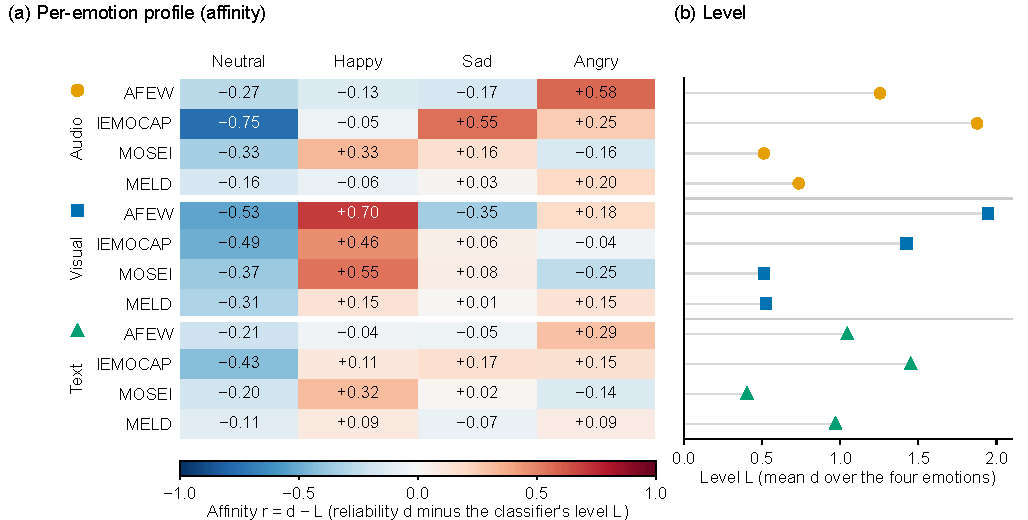
\includegraphics[width=0.8\linewidth]{fig7_strength_profile.pdf}
\paperfig{7}{各分類器の強さ（水準）はコーパスで入れ替わり，水準を引いた感情ごとの形（相性）はコーパスをまたいで似ていた．値は 4 コーパスを 1 つずつ仮のターゲットにした下調べ（K = 5）で測った．}
\end{figure}
\vspace{-3pt}
\zumiru{(a) は相性で，行は分類器（Audio ＝ 声，Visual ＝ 顔，Text ＝ 言葉）× コーパス，列は感情．赤はその感情が平均より得意，青は苦手を表す．顔の 4 行では Happy の欄が 4 コーパスとも赤く，Neutral の欄が 4 コーパスとも青い．(b) は水準で，同じモダリティでもコーパスによって大きく違う．}

\begin{itemize}
  \item \textbf{水準}：ソースで測った値と全ラベルで測った値の相関は −0.954〜+0.365，最も強いモダリティが一致した割合は 0〜0.367 だった．K 本で測った水準では，一致した割合が 0.433〜0.967 だった．
  \item \textbf{感情ごとの形}（表から水準と，どの分類器にも共通の感情ごとの当てやすさなどを除いた残り）：ソースの表と全ラベルの表の相関は 0.493〜0.770，感情の並びを入れ替えて元の相関以上になる割合は 0.096〜0.192 だった．K 本だけで測った表は，前もって決めた基準（相関 0.3 以上，入れ替えの割合 0.2 以下）をどのコーパスでも満たさなかった．
\end{itemize}
\begin{yowai}
これらは手法の形を決めるために使った下調べの値で，評価の回の値ではない．感情ごとに最も強いモダリティの順位が一致する基準を満たしたのは MOSEI だけである．
\end{yowai}
\noindent\textbf{結論}：水準はターゲットの K 本で測り，相性はラベルの多いソースのコーパスで測る．

%======================================================================
\pagesection{Q3：提案の手法（感情ごとの信頼度による late fusion）}\label{sec:q3method}
\koko{提案は，強さ（水準）をターゲットの K 本で，感情ごとの得意と不得意（相性）をソースで測った信頼度の表で 3 つの分類器の答えをまとめ，まとめた答えを疑似ラベルにする．}

\noindent\textbf{late fusion} は，声・顔・言葉の分類器を別々に学び，最後に答え（確率や点数）をまとめる方法である．Q1 の疑似ラベルは，3 つの確率を同じ重みで掛ける\textbf{積}でまとめた．提案は，積の代わりに感情ごとの信頼度の表で重みづけてまとめる．

\begin{figure}[H]
\centering
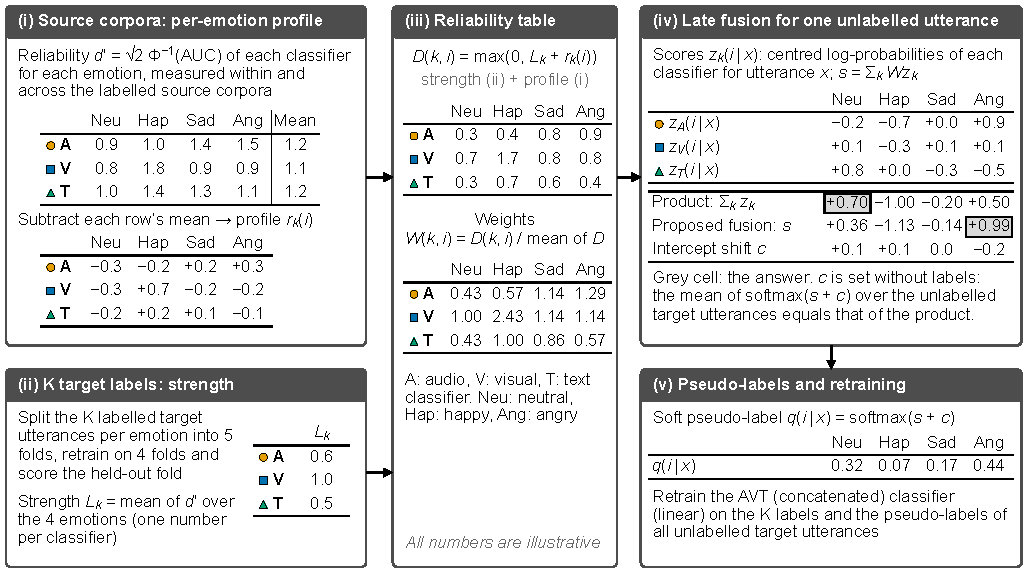
\includegraphics[width=0.82\linewidth]{fig8_method.pdf}
\paperfig{8}{感情ごとの信頼度による late fusion の手順（(i)〜(v)）．表の数値は説明のための例である．灰色の欄が答えで，例では積は Neutral（+0.70），提案は Angry（+0.99）を答える．}
\end{figure}
\vspace{-4pt}
\begin{center}
\small
\begin{tabular}{>{\raggedright}p{2.6cm}>{\raggedright\arraybackslash}p{13.6cm}}
\toprule
図の手順 & 中身（論文 7.2 節） \\
\midrule
(i) 相性（ソース） & ソースの中の話者で分けた交差検証で信頼度を測り，ほかのソースに当てたときに残る割合（\textbf{残り方}）を掛けてターゲットでの値を見込む．そこから行の平均を引く \\
(ii) 水準（K 本） & K 本を感情ごとに 5 組に分け，1 組ずつ抜いて学び直した分類器で抜いた組に点数を付け，信頼度の 4 感情の平均を水準にする（戻し先へ n0 本ぶん近づけてもよい） \\
(iii) 表と重み & 表 D(k, i) = max(0, 水準 + β × 相性)．12 個の平均で割って重み W(k, i) にする \\
(iv) まとめる & 点数 s(i | x) = Σ\textsubscript{k} W(k, i) × z\textsubscript{k}(i | x)（z は中心化した対数確率）．感情ごとに違う重みで答えが偏るので，ラベルを使わずに切片 c をずらす（ラベル無しの発話の上で確率の平均が積と同じになる点） \\
(v) 疑似ラベル & q = softmax(s + c) を候補に付け，融合の分類器（AVT．CREMA-D は AV）を Q1 と同じ損失で学び直す \\
\bottomrule
\end{tabular}
\end{center}
\begin{itemize}
  \item ハイパーパラメータは n0 ∈ \{0, 20, 80, ∞\}，β ∈ \{0, 1\}（相性を使うか），戻し先 2 つの 16 点で，仮のターゲットの 30 反復で選んだ．選ばれた点はどれも β = 1 で，n0 は 12 条件のうち 8 で 0，残りで 20 だった．n0 = ∞，β = 0 にすると積と同じ判定になる．
  \item \textbf{なぜ late fusion か}：Zadeh ほか 2017（TFN）は，late fusion はモダリティの間の関係を学べないと批判した．ラベルが感情ごとに数本しか無い設定では，答えの段でまとめると K 本から決める数を水準の 3 つにでき，感情ごとの形はラベルの多いソースで測れる．
  \item \textbf{先行研究との違い}（論文 2.4 節）：重みは発話ごとに学ぶ（M3ER，Marín ほか 2026）のではなく，分類器と感情の組ごとに 1 つ決める．まとめた答えを補助の課題（Self-MM）ではなく疑似ラベルに使う．調べた範囲では，信頼度の表を強さと形に分け，強さを K 本で，形をソースで測る組み立ては見つからなかった．
\end{itemize}

%======================================================================
\pagesection{Q3 の答え：提案は積を 12 条件のうち 11 で上回り，AFEW では 2.1〜3.5 点上げた}\label{sec:q3ans}
\toihead{cQ3}{Q3}{声・顔・言葉の分類器の答えを，疑似ラベルにするためにどうまとめればよいか．}
\begin{kotae}{cQ3}{Q3 の答え（論文 7 節の冒頭と 7.4 節）}
各分類器の強さ（水準）をターゲットの K 本で，感情ごとの得意と不得意の形（相性）をソースのコーパスで測った信頼度で 3 つの分類器の答えをまとめる late fusion（提案）は，確率の積を 4 コーパスの 12 条件のうち 11 で点推定で上回り，AFEW では UAR を 2.1〜3.5 点上げた．
\end{kotae}

\noindent\textbf{評価の設定}：4 コーパスを 1 つずつターゲットにし（ソースは残り 3 つ），50 反復．CREMA-D（声と顔）も評価した．\textbf{推定時の答え}はまとめた答えをそのまま感情の答えにしたもの，\textbf{学び直した融合の分類器}はまとめた答えを疑似ラベルにして学び直した分類器である．

\begin{figure}[H]
\centering
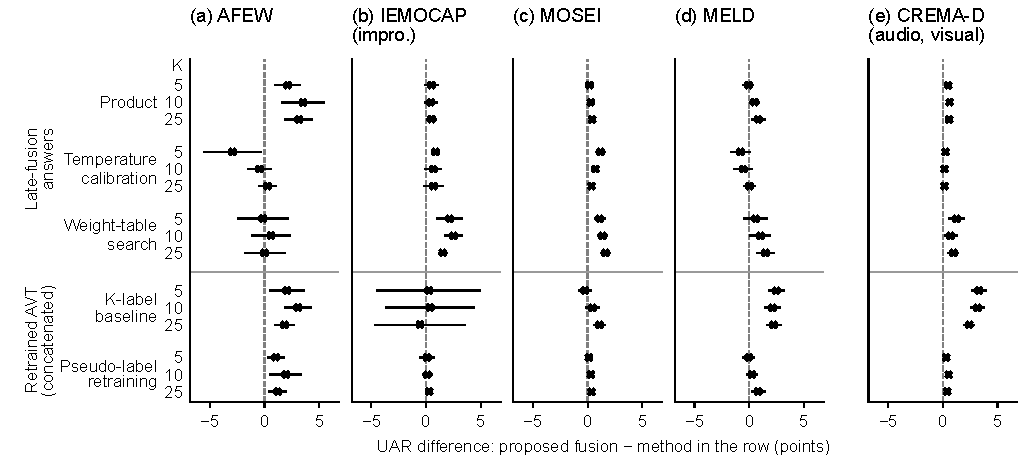
\includegraphics[width=0.84\linewidth]{fig9_fusion_vs_others.pdf}
\paperfig{9}{提案と比べる相手の UAR の差．AFEW の 3 つの K で区間が 0 を含まず 1.0 点以上で，IEMOCAP，MOSEI，MELD では −0.1〜+0.8 点だった．}
\end{figure}
\vspace{-4pt}
\zumiru{各点は提案 − 比べる相手の UAR の差で，0 より右なら提案が高い．上の 3 行（Inference）は推定時の答えどうし，下の 2 行（Retrained）は学び直した融合の分類器どうしの比べ．Product ＝ 積，Temperature calibration ＝ 分類器ごとの温度の較正，Weight-table search ＝ K 本で重みの表を探す方法（Kaya ほか 2017 の型），Fused, K labels only ＝ K 本だけの融合，Product pseudo-labels ＝ 積を疑似ラベルにした学び直し（Q1 の学び直し）．}

\begin{center}
\footnotesize
\begin{tabular}{llccc}
\toprule
比べ & コーパス & K = 5 & K = 10 & K = 25 \\
\midrule
\multirow{4}{3.4cm}{推定時の答え：\\提案 − 積} & \textbf{AFEW} & \textbf{+2.13} [+1.0, +3.3] & \textbf{+3.51} [+1.5, +5.5] & \textbf{+3.14} [+1.9, +4.4] \\
 & IEMOCAP & +0.49 [−0.2, +1.2] & +0.43 [−0.2, +1.1] & +0.50 [+0.01, +1.0] \\
 & MOSEI & +0.19 [−0.2, +0.6] & +0.29 [−0.03, +0.6] & +0.40 [+0.1, +0.7] \\
 & MELD & \textcolor{cTest}{−0.09} [−0.6, +0.4] & +0.48 [+0.01, +1.0] & +0.83 [+0.2, +1.5] \\
\midrule
\multirow{4}{3.4cm}{学び直した融合の分類器：\\提案 − Q1 の学び直し} & \textbf{AFEW} & \textbf{+1.01} [+0.2, +1.8] & \textbf{+1.95} [+0.5, +3.4] & \textbf{+1.21} [+0.4, +2.0] \\
 & IEMOCAP & +0.10 [−0.6, +0.8] & +0.13 [−0.3, +0.6] & +0.27 [−0.1, +0.6] \\
 & MOSEI & +0.10 [−0.2, +0.4] & +0.28 [−0.01, +0.6]＊ & +0.35 [+0.1, +0.6] \\
 & MELD & \textcolor{cTest}{−0.05} [−0.6, +0.5] & +0.25 [−0.2, +0.7] & +0.82 [+0.2, +1.5] \\
\bottomrule
\end{tabular}

\smallskip
{\scriptsize UAR の差（点）と 95\% 区間（論文の表 9）．AFEW の推定時の答えの UAR は，提案 71.36，74.39，76.58 に対し積 69.23，70.88，73.45．「12 条件のうち 11」は推定時の答えの点推定の符号で，負は MELD の K = 5 だけ．＊ は 0 を含むかどうかが引き直しの乱数に依りうる区間．}
\end{center}

\begin{yowai}
\begin{itemize}
  \item IEMOCAP，MOSEI，MELD の 9 条件の推定時の答えの差は −0.09〜+0.83 点で，区間が 0 を含まないのは IEMOCAP と MOSEI の K = 25 と MELD の K = 10・25 だけである．
  \item 手法の形と，学び直しと CREMA-D を評価に加えることは，同じテストの発話の上の下調べの結果を見た後に決め，固定してから評価を 1 回だけ計算した．このため，積を含む別のまとめ方との差は提案に有利な向きに偏りうる．
  \item CREMA-D（声と顔）では，表の 2 つの比べの差が +0.31〜+0.63 点で，6 つの区間はどれも 0 を含まなかった．ただし俳優が決まった 12 文を読み，同じ文が学習に使う発話とテストの両方に出るので，論文 7.4 節の感度の確かめと一緒に読む．
\end{itemize}
\end{yowai}

%======================================================================
\pagesection{Q3 の答え（続き）：差はどこから来たか，どの相手に提案が低かったか}\label{sec:q3cont}
\toihead{cQ3}{Q3}{提案と積の差は，水準と相性のどちらから，誤りのどの部分から来たのか．}

\noindent\textbf{AFEW で差が出た理由の候補}（論文 7.4 節．測っていない理由なので「1 つの可能な説明は」と書く）：AFEW では，3 つの分類器のうち顔の分類器だけの UAR が K = 5・10 で積より点推定で高く（70.70 対 69.23，71.93 対 70.88），50 反復と 4 感情で平均した提案の重みは 3 つの K とも顔が最大だった（K = 5 で顔 1.17，声 0.93，言葉 0.90）．「1 つの可能な説明は，1 つの分類器だけで積より UAR が高くなるコーパスでは同じ重みで掛ける積が UAR を下げ，提案は K 本で測った水準でその分類器を重くしたことである．」ほかの 3 コーパスでは，最も強い単独の分類器（IEMOCAP と MOSEI の声，MELD の言葉）の UAR は K = 5 で積より点推定で低かった（68.70 対 72.07，37.78 対 40.97，48.73 対 50.15．対の差の区間は作っていない）．

\medskip
\noindent\textbf{部品ごとの寄与}（論文 7.5 節．提案から部品を 1 つずつ外した版との差）
\begin{itemize}
  \item 提案 − 相性を外した版は 15 条件すべてで正（+0.10〜+0.73 点）だった．提案 − 分類器 × 感情の成分を消した版は 4 コーパスで +0.07〜+0.48 点だった．
  \item AFEW では，相性を外した版 − 積（+1.75，+3.06，+2.78）と，提案 − 分類器どうしの水準の違いを外した版（+1.74，+3.20，+2.57）が，3 つの K とも区間が 0 を含まず 1.0 点以上だった．
  \item MOSEI では，相性を外した版 − 積と提案 − 水準の違いを外した版が負で（−0.54〜−0.07．K = 5・10 は区間が 0 を含まない），提案 − 相性を外した版と水準の違いを外した版 − 積が正だった（+0.48〜+0.73．区間は 0 を含まない）．
\end{itemize}

\noindent\textbf{答えの偏りの分と重みの向きの分}（論文 7.6 節．\shiryo{sec:bunkai}の分け方を提案 − 積に当てた．計算の後に足した解析）
\begin{center}
\small
\begin{tabular}{lccc}
\toprule
量（推定時の答え，AFEW） & K = 5 & K = 10 & K = 25 \\
\midrule
全体（提案 − 積） & +2.13 [+1.0, +3.3] & +3.51 [+1.5, +5.5] & +3.14 [+1.9, +4.4] \\
重みの向きの分 & +2.55 [+1.1, +4.0] & +3.87 [+1.8, +5.9] & +3.35 [+2.1, +4.6] \\
切片の分（全体 − 向きの分） & −0.42 [−1.2, +0.3] & −0.36 [−1.1, +0.4] & −0.21 [−1.0, +0.6] \\
\bottomrule
\end{tabular}
\end{center}
\noindent 切片の分は 4 コーパスの 12 条件とも区間が 0 を含んだ（−0.42〜+0.17 点）．提案 − 積の差は重みの向きの分に現れた．Q2 で，ほかのモダリティの疑似ラベルが減らしたのも重みの向きのずれだった．

\begin{yowai}[提案が低かった相手と，上がらなかった試み]
\begin{itemize}
  \item 区間が 0 を含まずに提案が低かったのは，切片をずらした答えどうしでは，分類器ごとの温度の較正との差の AFEW の K = 5（−2.94 [−5.6, −0.3]，71.36 対 74.30）だけだった．表 9 に無い相手では，K 本で合わせたモダリティごとの重みとの差が AFEW で −3.54〜−1.50 点だった（区間は 0 を含む）．
  \item 区間が 0 を含まずに提案が部品を外した版より低いのは，水準を戻さない版との差の AFEW と MELD の K = 5，残り方を掛けない版との差の IEMOCAP の K = 25 と CREMA-D の K = 5・10，水準の違いを外した版との差の MOSEI の K = 5・10 である．
  \item K 本で推した取り違えの表で疑似ラベルを補正する方法（Gold Loss Correction）は，K = 5 で Q1 の学び直しの UAR を上げなかった．MOSEI の声では，候補の全ラベルで数えた表での補正は補正しない版を +0.8 点 [+0.1, +1.6] 上回ったので，上がらなかったのは K 本（20 本）からの表の推定の不足による．
\end{itemize}
\end{yowai}

%======================================================================
\pagesection{新しいコーパスで，手間をどこに回すか}\label{sec:tema}
\koko[\ess{6}]{論文の結果を，新しいコーパスで MER の分類器を作る人が手間をどこに回すかの判断の材料に言い直す（論文 8.4 節）．}

\begin{figure}[H]
\centering
\begin{tikzpicture}[tb/.style={draw,rounded corners=3pt,align=left,font=\small,inner sep=5pt,text width=4.6cm,minimum height=2.5cm},
  nb/.style={draw=black!40,fill=white,rounded corners=2pt,align=left,font=\footnotesize,inner sep=4pt,text width=4.9cm,minimum height=2.5cm}]
  \node[font=\small\bfseries] at (2.5,3.0) {直す誤りの部分};
  \node[font=\small\bfseries] at (8.0,3.0) {手間の回し方（論文 8.4 節）};
  \node[font=\small\bfseries] at (13.6,3.0) {根拠の数値};
  % 1
  \node[tb,fill=cQ2!5] (a1) at (2.5,1.4) {\textbf{第 1：答えの偏り}\\答えが一部の感情に偏る誤り．切片を動かせば直る};
  \node[tb,fill=cGood!8,text width=4.9cm] (b1) at (8.0,1.4) {特徴をコーパスごとに標準化（平均を引く）すれば，ラベル無しで直る．ラベルはまず要らない};
  \node[nb] (c1) at (13.6,1.4) {平均を引く方法の gain は声で +4.69 点，合併は +5.26 点（単一ソース設定，K = 5．\shiryo{sec:q2bias}）};
  % 2
  \node[tb,fill=cQ2!5] (a2) at (2.5,-1.4) {\textbf{第 2：残りの誤り}\\偏りを除いても残る誤り．重みを変えないと直らない};
  \node[tb,fill=cGood!8,text width=4.9cm] (b2) at (8.0,-1.4) {ラベルを数本増やしても遅くしか減らない．声・顔・言葉のそろうラベル無しの録画を集め，ほかのモダリティの疑似ラベルで学び直す};
  \node[nb] (c2) at (13.6,-1.4) {K 本だけの向きの良さは声で K = 5 のとき 0.47．疑似ラベルは 81 条件のうち 38 で残りの誤りを減らした．学び直した声の UAR は K = 5 のとき +2.4〜+4.1 点（\ref{sec:q1ans}・\ref{sec:q2bias}・\ref{sec:q2pl} 節）};
  % 3
  \node[tb,fill=cQ3!6] (a3) at (2.5,-4.2) {\textbf{第 3：答えのまとめ方}\\3 つの分類器の答えを疑似ラベルにまとめる};
  \node[tb,fill=cGood!8,text width=4.9cm] (b3) at (8.0,-4.2) {強さを数本のラベルで測り直す．ターゲットで最も強いモダリティがソースと違うとき（論文では AFEW の顔），同じ重みの積との差が大きく出た};
  \node[nb] (c3) at (13.6,-4.2) {AFEW で提案 − 積は +2.13〜+3.51 点．ほかの 3 コーパスでは −0.09〜+0.83 点（\shiryo{sec:q3ans}）};
  \foreach \i in {1,2,3}{ \draw[arr] (a\i) -- (b\i); \draw[arr] (b\i) -- (c\i); }
\end{tikzpicture}
\caption{論文の結果から言える，手間の回し方．範囲は，凍結した特徴の上の線形分類器と，論文の 4〜7 群のコーパスでの観察である．}
\end{figure}

\noindent 論文は，この判断を要旨の最後の文と序論の最後に置いている：「これらの結果は，新しいコーパスで MER の分類器を作るときに，手間をラベル付けに回すか，ラベル無しのマルチモーダルの録画に回すかを決める材料になる．」

\begin{waku}{手本にした書き方（エッセンス 6：読者が持ち帰る判断を書く）}
\small
\begin{itemize}
  \item Hayashi 2025（岡田先生・石井さんの共著）は，1 つ目の研究目的が「性格の情報を集める費用に見合うだけ推定が上がるかを，読者が判断する材料になる」と書く．
  \item Okada 2019 は，枠組みを使うための指針を示す．
  \item 論文は同じ形で，「新しいコーパスでラベル付けとラベル無しの録画のどちらに手間を回すか」を読者が持ち帰る判断にした．範囲（凍結した特徴，線形分類器，この実験の範囲）は主張の文の中に入れ，後から断り書きを足さない．
\end{itemize}
\end{waku}

%======================================================================
\pagesection{限界と，理解のための第一歩}\label{sec:genkai}
\koko[\ess{2}]{結果を読むときの範囲と，次に確かめることを，論文 9 節の 7 つの段落から短くまとめる．}

\begin{center}
\small
\begin{tabular}{>{\raggedright}p{3.4cm}>{\raggedright}p{6.5cm}>{\raggedright\arraybackslash}p{6.3cm}}
\toprule
限界（論文 9 節の見出し） & 中身 & だから結果をどう読むか・次に試すこと \\
\midrule
設定とコーパスの範囲 & 6.1〜6.3 節は単一ソース設定，6.4 節は全ソース設定，5，6.5，7 節は LOCO 設定の結果．エンコーダは各モダリティに 1 組ずつ（声だけ HuBERT も）．8 種類の特徴は同じコーパス・話者・分割の上で計算した & 8 節の答えは設定の違う結果を並べたもので，8 種類の特徴は独立な再現ではない．ほかのコーパス（MSP-IMPROV など）とほかのエンコーダで次に確かめる \\
凍結した特徴と線形の分類器 & 結果は凍結した特徴の上の線形分類器についての結果．微調整すると凍結した特徴より高い UAR が得られることが報告されている & 微調整した場合に偏りと残りの誤りの分かれ方が同じになるかは分からない \\
同じデータの上で立てた説明と作った手法 & 3 つの条件は Q1 の結果を見た後に立てた．手法の形，格子，選び方は評価に使ったコーパスの上で作った & 積などとの差は提案に有利な向きに偏りうる．新しいコーパスで，手順を固定したまま 1 回だけ評価することが次の段階 \\
疑似ラベルに含まれる自分のモダリティ & 疑似ラベルは学び直す分類器自身のモダリティの予測も含む & 学び直しの gain をほかのモダリティの情報だけに帰すことはできない \\
テストと学習の内容の共有 & 話者は分けたが，MOSEI では同じ人物の別の動画，MELD では同じ回，IEMOCAP の即興では同じ筋書きが両方に現れうる & IEMOCAP の言葉の分類器の gain は，筋書きの話題の共有と分けられなかった \\
誤りの分け方の模型 & 残りの誤りは，2 つの感情の点数を分散の等しい正規分布とみなす模型の上の量 & 単一ソース設定では偏りの分を模型ではなく UAR で測った．直る速さの曲線は K $\le$ 10 の要約で，仮定のうち 2 つは満たされなかった \\
中間層の値は再現の量 & 論文 6.6 節は候補の上で疑似ラベルの判定を再現できる量を測った & 中間層の特徴で学び直した分類器のテストの UAR は測っていない．取り戻した分には言葉の内容や録音の環境の手がかりも入りうる \\
\bottomrule
\end{tabular}
\end{center}

\noindent 論文の書き方：区間が 0 を含む条件は結果の節の中に数値で書き（この資料の赤い枠），限界の節では短い見出しの段落で並べて，長い断りを繰り返さない．Kikuchi 2026 と Sakuramoto 2026（岡田研）の限界の書き方に倣った．

\begin{kotae}{cQ2}{論文の結び（10 節の最後の文）}
本研究は，新しいコーパスで MER の分類器を作るときに，どの情報源が分類器のどの誤りを直すのかを理解するための第一歩である．
\end{kotae}
\noindent この結び方は，既知の結果を土台にして「なぜ」を問う論文の結び方である（エッセンス 2．Hayashi 2025 などの ``the first step toward understanding why ...''）．結論の段落は，何をして何が分かったかを数値つきで 1 段落に書く（声の分類器は 12 条件すべてで上がり，K = 5（感情ごとに 5 本のラベル）のとき 2.4〜4.1 点，声の特徴は言葉の分類器の判断を顔の特徴より 14.9〜16.7 点よく再現，提案は積を 12 条件のうち 11 で上回り，AFEW で 2.1〜3.5 点）．

%======================================================================
\pagesection{この論文の書き方 (1)：岡田先生・石井さんの 6 つのエッセンス}\label{sec:kakikata}
\koko{岡田先生（JAIST）と石井さん（NTT）の論文 16 本から取り出した 6 つのエッセンスを，論文のどこにどう使ったか，この資料のどこで使ったかを示す．}

\noindent 2 人は，文ごとに語を弱めるのではなく，\textbf{主張の強さを問いの立て方と証拠の種類で決める}．証拠があるところは言い切る（Ishii 2022 の ``critically important''，Okada 2019 の ``more accurate than previous models for 14 out of 15 traits''）．

\begin{center}
\footnotesize
\begin{tabular}{>{\raggedright}p{2.9cm}>{\raggedright}p{4.0cm}>{\raggedright}p{6.6cm}>{\raggedright\arraybackslash}p{2.1cm}}
\toprule
エッセンス & 岡田先生・石井さんの論文での形 & この論文での使い方 & この資料 \\
\midrule
\textbf{1} 問題を，方法からではなく人や場面の側から立てる & Ishii 2022 は「円滑な会話のために参加者は相手の意欲を見て振る舞いを変えなければならない」から始める．Sakuramoto 2026 は実環境の性質から始める & 序論 1 段落目「MER のコーパスは，感情をどう引き出し，どう録り，どうラベルを付けたかが互いに違う．」2 段落目でラベルの費用（複数の評定者）を書き，分類器の成績はその後に置く & \ref{sec:bamen} 節 \\
\textbf{2} 新しさを「知られていることが，この場面でも成り立つか」で立てる & Hayashi 2025 は，初対面の相手で推定を上げた性格の情報が，友人どうしでも推定を上げるかを問う．最後は ``the first step toward understanding why ...'' で結ぶ & 序論 3 段落目：Albanie ほか 2018 の既知の結果 →「しかし，新しいコーパスに感情ごとに数本のラベルしか無いときにも，…まだ分かっていない．」結論の最後は「…理解するための第一歩である．」 & \ref{sec:toi} 節，\ref{sec:genkai} 節 \\
\textbf{3} 問いを番号で立て，主張は問いへの答えとして書く．範囲は主張の文の中に入れる & Ishii 2022 は Q1，Q2-1，Q2-2 を立て，手法を ``To address Q1''，考察を ``Answer to Q1'' で書く．図 1 は ``Overview of our research questions'' & 序論に Q1〜Q3 を疑問文で置き，図 1 を問いの概観にした．5〜7 節の見出しを答えの文にし（例：「5 ほかのモダリティを含む疑似ラベルで学び直すと，声の分類器の UAR は 12 条件すべてで上がった」），8 節の小見出しを「8.1 Q1 への答え：…」にした & \ref{sec:toi} 節，各頁の見出しの Q1〜Q3 \\
\textbf{4} 「上がるか」の次に「なぜ上がるか」を，量を成分に分けて答える & Hayashi 2025 はラポールの評定を 3 成分（評定する人の癖，評定される人の印象，その 2 人の組だけの関係）に分け，どの入力がどの成分を捉えたかを示す．Kikuchi 2026 は 2 つの予測が重なる分散を測ってから「補い合う」と言う & 4 節で誤りを答えの偏り（切片のずれ）と残りの誤り（重みの向きのずれ）に分け，6 節で 4 つの情報源がどちらを直すかを同じ分け方で測った．7.6 節では提案 − 積の差も同じ分け方で分けた & \ref{sec:bunkai}，\ref{sec:q2all}，\ref{sec:q3cont} 節 \\
\textbf{5} 動詞の強さを証拠の種類に合わせる & ``Our results show''（自分の観察は過去形），``suggesting that''，``one possible explanation is''，``have been reported'' & 次の頁の表のとおり．区間が 0 を含む条件は結果の節の中に数値で書く & 各頁の赤い枠，\ref{sec:q1cont}，\ref{sec:q3cont}，\ref{sec:doushi} 節 \\
\textbf{6} 読者が持ち帰る判断を書く & Hayashi 2025 は「性格の情報を集める費用に見合うか判断する材料」を書く．Okada 2019 は枠組みを使う指針を示す & 要旨の最後の文と序論の最後：「…手間をラベル付けに回すか，ラベル無しのマルチモーダルの録画に回すかを決める材料になる．」8.4 節で 3 つの判断に分けた & 表紙，\ref{sec:tema} 節 \\
\bottomrule
\end{tabular}
\end{center}

\begin{waku}{文のつなぎ：各文の頭で，前の文の最後の語を受ける（要旨 第 7 版の流れ）}
\small
\begin{tikzpicture}[lb/.style={draw=black!50,fill=white,rounded corners=2pt,font=\scriptsize,align=center,inner sep=3pt,text width=1.95cm,minimum height=1.25cm}]
  \node[lb] (1) at (0,0) {コーパスごとに違い，\\ほかのコーパスで\\成績が落ちる};
  \node[lb] (2) at (2.35,0) {合わせるには\\ラベルが要るが\\費用がかかる};
  \node[lb] (3) at (4.7,0) {この費用を減らす\\ため，疑似ラベルが\\使われてきた};
  \node[lb] (4) at (7.05,0) {しかし，数本の\\ときに上がるか\\…分かっていない};
  \node[lb] (5) at (9.4,0) {これらの問いに\\答えるため，\\誤りを 2 つに分けた};
  \node[lb] (6) at (11.75,0) {その結果 …\\これをもとに\\提案する};
  \node[lb,fill=cGood!8] (7) at (14.1,0) {手間をどこに\\回すかを決める\\材料になる};
  \foreach \a/\b in {1/2,2/3,3/4,4/5,5/6,6/7}{ \draw[arr] (\a) -- (\b); }
\end{tikzpicture}
\end{waku}

%======================================================================
\pagesection{この論文の書き方 (2)：動詞の強さを証拠の種類に合わせる}\label{sec:doushi}
\koko[\ess{5}]{論文は証拠の種類ごとに使う動詞を決めている．自分で測った結果か，そこからの解釈か，測っていない理由かで書き方が変わる．}

\begin{center}
\small
\begin{tabular}{>{\raggedright}p{3.0cm}>{\raggedright}p{3.2cm}>{\raggedright\arraybackslash}p{9.7cm}}
\toprule
証拠の種類 & 使う動詞 & 論文の例（日本語の下書き） \\
\midrule
自分で測った結果 & 「示す」．観察は過去形（「〜だった」「〜が減った」） & 「表 4 と図 3 は，K = 5 で声の分類器の UAR が 4 コーパスすべてで K 本だけの分類器より高かったことを示す．」（5.3 節） \\
測った結果からの解釈 & 「示唆する」 & 「これらの結果は，表 4 の声の gain が，損失の形にも仮のターゲットでのハイパーパラメータの選択にもよらず，学び直す分類器の損失に q を加えることから生じたことを示唆する．」（5.5 節） \\
測っていない理由 & 「1 つの可能な説明は〜」 & 「1 つの可能な説明は，音声には声の調子に加えて話している言葉の手がかりも入っているので，声の分類器は言葉の側から来た判断の一部を自分の特徴で学べる，というものである．」（8.2 節） \\
原因の候補 & 「〜しうる」（「〜ので」と断定しない） & 「このため，積を含む別のまとめ方との差は提案に有利な向きに偏りうる．」（7.3 節） \\
言えないこと & 「〜とは言えない」「〜までは言えない」 & 「声だけがほかのモダリティの手がかりを持つとは言えない．」（6.5 節）「声の特徴に言葉の中身が入っているとまでは言えない．」（8.2 節） \\
他人の結果 & 「報告されている」 & 「1 つのコーパスで学んだ MER の分類器は，ほかのコーパスでは成績が落ちることが報告されている．」（1 節） \\
先行研究と合う & 「〜と同じ向きである」 & 「本研究の結果はこれと同じ向きであり，…声の分類器ではほかのモダリティの予測が学習の目標として働くことを示している．」（8.1 節） \\
設定 & 「本研究は〜の場合を考える」 & 「本研究は，新しいコーパス（ターゲット）に感情ごとに数本のラベルしか無い場合を考え，…」（1 節） \\
\bottomrule
\end{tabular}
\end{center}

\begin{waku}{使わない言い方}
\small
\begin{itemize}
  \item 程度を形容詞や副詞で言わない（「大きく」「顕著に」）．要旨と序論の成果は具体的な数値で書く（「K = 5 では 2.4〜4.1 点上がった」「12 条件のうち 11 で上回った」）．
  \item 測っていない頻度を言わない（「多くの場合」「ふつう」）．範囲を付けずに「初めて」と言わない．論文は「調べた範囲では，…組み立ては見つからなかった」と書く．
  \item 結果に「探索」のラベルを付けない．実験の番号を本文に書かない．
  \item 区間が 0 を含む条件は結果の節の中に数値で書き，限界の節で長い断りを繰り返さない．
  \item 差が有意でないことから強い結論を出さない．検定を示さずに「有意に」と書かない（2 人の論文の中でも手本にしなかった点）．
\end{itemize}
\end{waku}

\begin{waku}{この資料で使った言葉}
\footnotesize
\begin{tabular}{@{}>{\raggedright}p{3.6cm}>{\raggedright\arraybackslash}p{12.4cm}@{}}
ソース／ターゲット & ラベルが全部ある既存のコーパス／ラベルが少ない新しいコーパス \\
K 本，候補 & 感情ごとにラベルを使う本数（K = 5 なら計 20 本）／ターゲットのテスト以外の発話（K 本以外はラベルを使わない） \\
疑似ラベル（q），積 & 分類器が付けたラベル（4 感情の確率のまま使う）／3 つの分類器の確率を同じ重みで掛けるまとめ方 \\
アンカー & 学び直すときに重みと切片を引き戻す先の分類器（L2 正則化の中心） \\
答えの偏り／残りの誤り & 切片のずれ（切片を動かせば直る）／重みの向きのずれ（重みを変えないと直らない） \\
余地，当たる幅 Δ，再現できる分 P & 学び直しで UAR が上がる 3 つの条件を測る量（\shiryo{sec:q2cond}） \\
信頼度，水準，相性 & 分類器 × 感情ごとの見分けやすさ／その 4 感情の平均／平均との差 \\
提案 & 水準を K 本で，相性をソースで測った信頼度の表で 3 つの分類器の答えをまとめる late fusion \\
仮のターゲットの回／評価の回 & ソースの 1 つをターゲットに見立ててハイパーパラメータを選ぶ計算／選んだ設定で 1 回だけ測る計算 \\
\end{tabular}
\end{waku}

\end{document}
